\documentclass[a4paper,pdftex,10pt]{article}
\usepackage[a4paper]{geometry}
\usepackage[utf8]{inputenc}
\usepackage[T1]{fontenc} 
\usepackage[english,slovene]{babel} 
\usepackage{amsmath,amsfonts,amsthm,amssymb,mathrsfs,empheq} % Math packages
\usepackage{mathtools}
\usepackage{dsfont}
\usepackage{wrapfig}
\usepackage[pdftex]{graphicx}
%\usepackage{makeidx}
\usepackage{url}
\usepackage{caption}
\usepackage{subcaption}
\usepackage{tabularx}
\usepackage{float}

\usepackage[version=3]{mhchem} %kemija


\renewcommand{\vec}[1]{\boldsymbol{\mathbf{#1}}}                                        
\newcommand{\ihat}[0]{\boldsymbol{\mathbf{\oldhat{\textbf{\i}}}}} % pokončna j in i (j i n i
\newcommand{\iu}{{i\mkern1mu}}	    %imaginarno število
\DeclarePairedDelimiterX{\norm}[1]{\lVert}{\rVert}{#1} %norma

\usepackage{fancyhdr} % Custom headers and footers
\pagestyle{fancyplain} % Makes all pages in the document conform to the custom headers and footers
\fancyhead{} % No page header - if you want one, create it in the same way as the footers below
\fancyfoot[L]{} % Empty left footer
\fancyfoot[C]{} % Empty center footer
\fancyfoot[R]{\thepage} % Page numbering for right footer
\renewcommand{\headrulewidth}{0pt} % Remove header underlines
\renewcommand{\footrulewidth}{0pt} % Remove footer underlines
\setlength{\headheight}{13.6pt} % Customize the height of the header

%\numberwithin{equation}{section} % Number equations within sections (i.e. 1.1, 1.2, 2.1, 2.2 instead of 1, 2, 3, 4)
\numberwithin{figure}{section} % Number figures within sections (i.e. 1.1, 1.2, 2.1, 2.2 instead of 1, 2, 3, 4)
%\numberwithin{table}{section} % Number tables within sections (i.e. 1.1, 1.2, 2.1, 2.2 instead of 1, 2, 3, 4)

\setlength\parindent{0pt} % Removes all indentation from paragraphs - comment this line for an assignment with lots of text

%----------------------------------------------------------------------------------------
%	TITLE SECTION
%----------------------------------------------------------------------------------------

\newcommand{\horrule}[1]{\rule{\linewidth}{#1}} % Create horizontal rule command with 1 argument of height

\title{	
\normalfont \normalsize 
\textsc{Modelska analiza 1} \\ [25pt] % Your university, school and/or department name(s)
%\horrule{0.2pt} \\[0.4cm] % Thin top horizontal rule
\huge 7. naloga - Integracije z metodo Monte Carlo\\ % The assignment title
%\horrule{0.2pt} \\[0.5cm] % Thick bottom horizontal rule
}

\author{Tina Klobas} % Your name

\date{\normalsize\today} % Today's date or a custom date

\begin{document}

\maketitle % Print the title

\section{Opis problema}
Metoda Monte Carlo sloni na vzorčenju naključnih dogodkov s~čimer potem dobimo 
dober numerični približek za izbrano količino. Za različne probleme je potek metode
enak: najprej omejimo območje možnih vnosov, naključno izberemo elemente iz omejene domene,
ki sledijo določeni verjetnostni porazdelitvi, obdelamo podatke in pogledamo ugodne
in neugodne izide. V~tej nalogi se ukvarjamo predvsem z~numeričnim integriranjem, za kar
uporabimo približek
\begin{equation} \label{Monte}
    \theta = \int_{\Omega} \!g(x) f(x) \,\text{d}V = V \hat{\theta}
    \pm V \frac{ \sigma_{\hat{\theta}} }{\sqrt{N}} 
\end{equation}
kjer je $V$ volumen območja $\Omega$ in $\sigma_{\hat{\theta}}^2 = 
\hat{\theta^2} - \hat{\theta}^2 $. Velja 
\begin{equation} \label{Carlo}
    \hat{\theta} = \frac{1}{N} \sum_{i=1}^N g(x_i), \quad
    \hat{\theta^2} = \frac{1}{N} \sum_{i=1}^N g^2(x_i)
\end{equation}
kjer so naključna števila $x_i$ z~območja $\Omega$ porazdeljena po verjetnostni gostoti
$f(x)$.
\pagebreak
%----------------------------------------------------------------------------------------
%	PROBLEM 1
%----------------------------------------------------------------------------------------
\section{Omejeno telo}
Telo omejimo s~ploskvijo
\begin{equation}
    \sqrt{|x|} + \sqrt{|y|} + \sqrt{|z|} = 1
\end{equation}
in določimo njegov vztrajnostni moment ter maso v~dveh primerih:
\begin{itemize}
    \item če je gostota $\rho = \rho_0$,
    \item če je gostota $\rho = r^p $, kjer je $r$ razdalja od središča telesa,
	$p$ pa poljuben parameter.
\end{itemize}

\begin{figure}[!]
    \centering
	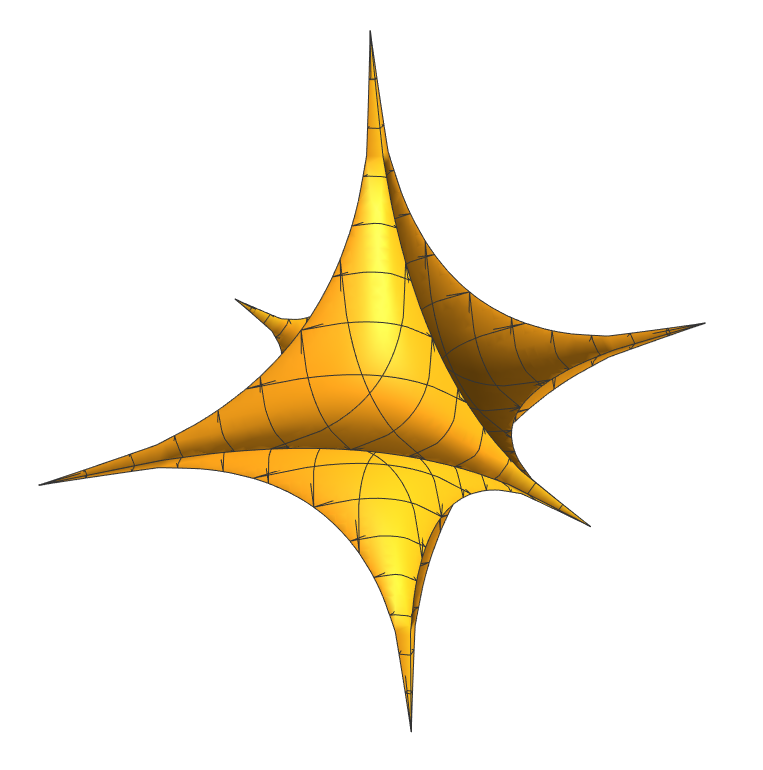
\includegraphics[width=.5\linewidth]{zvezda}
	\label{zvezda}
    \caption{Slika telesa, ki ga omejuje podana ploskev.}
\end{figure}

\subsection{Računanje volumna}
Volumen izračunamo z~integralom po območju volumnu $V'$ $\Omega$, ki predstavlja kar
volumen telesu očrtane kocke
\begin{equation} \label{volumen}
    V = \int_{\Omega} \!h(x,y,z) \,\text{d}V' \approx V' \hat{V} \pm V' 
    \frac{\sigma_{\hat{V}}}{\sqrt{N}}
\end{equation}
kjer je $h$ funkcija kombinacij naključnih števil $x_i, \, y_i, \, z_i$ iz kocke 
$ \Omega = [-1,1] \times [-1,1] \times [-1,1]$ ali pa iz krogle z~radijem $R=1$:
\begin{equation}
    h(x,y,z) = \left\{
	\begin{split}
	    &1; \quad \text{če } x^2 + y^2 \leq 1, y^2+z^2 \leq 1 \text{ in }
	    z^2+z^2 \leq 1 , \\
	    &0; \quad \text{sicer},
	\end{split}
    \right.
\end{equation}
s~čimer lahko nadalje poenostavimo
\begin{align}
    \hat{V} = \frac{1}{N} \sum_{i=1}^{N} h(x_i,y_i,z_i) = \frac{n}{N}, \\
    \hat{V^2} = \frac{1}{N} \sum_{i=1}^{N} h^2(x_i,y_i,z_i) = \frac{n}{N},
\end{align}
kjer je $n$ število vseh ugodnih kombinacij. Iz tega lahko izračunamo še varianco 
$\sigma_{\hat{V}}$:
\begin{equation}
    \sigma_{\hat{V}}^2 = \hat{V^2} - \hat{V}^2 = \frac{n(N-n)}{N^2}
\end{equation}
in končno lahko za prostornino~\ref{volumen} zapišemo približek:
\begin{equation} \label{prostornina}
    V = V' \hat{V} \pm V' \frac{\sigma_{\hat{V}}}{\sqrt{N}} = 
    V' \frac{n}{N} \left(1  \pm \sqrt{\frac{1}{n} - \frac{1}{N}} \right).
\end{equation}
($V'=8$ za kocko in $V'=\pi$ za kroglo.)

\subsection{Računanje vztrajnostnih momentov}
Tenzor vztrajnostnega momenta zapišemo kot
\begin{equation} \label{tenzor}
    J = \iiint_{\Omega} \!\rho(\vec{r}) \left(r^2 \mathds{1} - \vec{r} \otimes \vec{r} 
    \right) \,\text{d}V.
\end{equation}
Diagonalne komponente v~našem primeru so zaradi simetričnosti telesa enake
\begin{equation}
    J_{xx} = J_{yy} = J_{zz} = \int \!\rho (y^2 + z^2) \,\text{d}V,
\end{equation}
za izvendiagonalne komponente pa velja $J_ij=J_ji$ kjer je npr.
\begin{equation}
    J_{xy} = - \int \!\rho (-xy) \,\text{d}V.
\end{equation}
Po enačbi~\ref{Carlo} lahko potem zapišemo
\begin{equation}\label{Jxx}
    J_{xx} = \frac{V'}{N} \sum_{i=1}^N (y_i^2 + z_i^2) \rho(\vec{r}) h(x_i,y_i,z_i)
\end{equation}
in analogno za ostale integrale. 

\subsubsection{Izbira koordinat}
Komponente $x_i, y_i, z_i$ izžrebamo enakomerno z~intervala $[-1,1]$:
\begin{align}
    x &\sim u(-1,1), \nonumber\\
    y &\sim v(-1,1), \\
    z &\sim w(-1,1). \nonumber 
\end{align}
Če želimo uporabiti sferične koordinate, moramo upoštevati pretvorbo spremenljivk - velja:
\begin{equation}
    \frac{\mathrm{d} P}{\mathrm{d} V} = \frac{\mathrm{d}^3 P}{\mathrm{d}\varphi \mathrm{d}
    (\cos\vartheta) r^2 \mathrm{d}r} = \frac{1}{4\pi r^2},
\end{equation}
oziroma po posameznih spremenljivkah
\begin{align}
    \frac{\mathrm{d} P}{\mathrm{d} \varphi} &= \frac{1}{2\pi}, \nonumber\\ 
    \frac{\mathrm{d} P}{\mathrm{d} (\cos\vartheta)} &= \frac{1}{2}, \\ 
    \frac{\mathrm{d} P}{\mathrm{d} r} &=  \frac{\mathrm{d} P}{\mathrm{d} m} 
    \frac{\mathrm{d} m}{\mathrm{d} r} = \frac{\rho(r) 4\pi r^2}{M}. \nonumber
\end{align}
Če upoštevamo še enakomerno porazdelitev $\mathrm{d} P/\mathrm{d}u_i =1$ dobimo recept
za izbor enakomerne porazdelitve v~sferičnih koordinatah:
\begin{align}
    \varphi &\sim 2\pi u_1, \nonumber\\
    \vartheta &\sim \arccos(2u_2-1), \\
    r &\sim \sqrt[3+p]{u_3}. \nonumber
\end{align}
kjer so $u_1,u_2,u_3$ enakomerno izbrane z~intervala $(0,1)$. V~tem primeru moramo paziti
saj integriramo po volumnu krogle ($V'=4\pi$).

\subsection{Rezultati}
\subsubsection{Volumen}
Volumen telesa izračunan z~$n=10^5$ točkami:
$$V = 0,0891 \pm 0,0003.$$
%$$\tilde{V} = 8(2 - \sqrt{2}) \approx 4,686. $$ 
Da je $10^5$ točk dovolj lahko razberemo tudi z~grafa~\ref{slika3}, kjer vidimo, da se 
rezultat že okoli tisoč točk ustali; njegova relativna napaka je takrat reda $10^{-2}$
pri deset tisoč točkah pa samo še $10^{-3}$. Narisana je še krivulja $f(N) = 1/\sqrt{N}$,
ki se ji točke (razen začetnih nekaj) zelo lepo prilagajajo.\\
\begin{figure}    
    \centering
    \resizebox{.49\linewidth}{!}{% GNUPLOT: LaTeX picture with Postscript
\begingroup
  \makeatletter
  \providecommand\color[2][]{%
    \GenericError{(gnuplot) \space\space\space\@spaces}{%
      Package color not loaded in conjunction with
      terminal option `colourtext'%
    }{See the gnuplot documentation for explanation.%
    }{Either use 'blacktext' in gnuplot or load the package
      color.sty in LaTeX.}%
    \renewcommand\color[2][]{}%
  }%
  \providecommand\includegraphics[2][]{%
    \GenericError{(gnuplot) \space\space\space\@spaces}{%
      Package graphicx or graphics not loaded%
    }{See the gnuplot documentation for explanation.%
    }{The gnuplot epslatex terminal needs graphicx.sty or graphics.sty.}%
    \renewcommand\includegraphics[2][]{}%
  }%
  \providecommand\rotatebox[2]{#2}%
  \@ifundefined{ifGPcolor}{%
    \newif\ifGPcolor
    \GPcolortrue
  }{}%
  \@ifundefined{ifGPblacktext}{%
    \newif\ifGPblacktext
    \GPblacktexttrue
  }{}%
  % define a \g@addto@macro without @ in the name:
  \let\gplgaddtomacro\g@addto@macro
  % define empty templates for all commands taking text:
  \gdef\gplbacktext{}%
  \gdef\gplfronttext{}%
  \makeatother
  \ifGPblacktext
    % no textcolor at all
    \def\colorrgb#1{}%
    \def\colorgray#1{}%
  \else
    % gray or color?
    \ifGPcolor
      \def\colorrgb#1{\color[rgb]{#1}}%
      \def\colorgray#1{\color[gray]{#1}}%
      \expandafter\def\csname LTw\endcsname{\color{white}}%
      \expandafter\def\csname LTb\endcsname{\color{black}}%
      \expandafter\def\csname LTa\endcsname{\color{black}}%
      \expandafter\def\csname LT0\endcsname{\color[rgb]{1,0,0}}%
      \expandafter\def\csname LT1\endcsname{\color[rgb]{0,1,0}}%
      \expandafter\def\csname LT2\endcsname{\color[rgb]{0,0,1}}%
      \expandafter\def\csname LT3\endcsname{\color[rgb]{1,0,1}}%
      \expandafter\def\csname LT4\endcsname{\color[rgb]{0,1,1}}%
      \expandafter\def\csname LT5\endcsname{\color[rgb]{1,1,0}}%
      \expandafter\def\csname LT6\endcsname{\color[rgb]{0,0,0}}%
      \expandafter\def\csname LT7\endcsname{\color[rgb]{1,0.3,0}}%
      \expandafter\def\csname LT8\endcsname{\color[rgb]{0.5,0.5,0.5}}%
    \else
      % gray
      \def\colorrgb#1{\color{black}}%
      \def\colorgray#1{\color[gray]{#1}}%
      \expandafter\def\csname LTw\endcsname{\color{white}}%
      \expandafter\def\csname LTb\endcsname{\color{black}}%
      \expandafter\def\csname LTa\endcsname{\color{black}}%
      \expandafter\def\csname LT0\endcsname{\color{black}}%
      \expandafter\def\csname LT1\endcsname{\color{black}}%
      \expandafter\def\csname LT2\endcsname{\color{black}}%
      \expandafter\def\csname LT3\endcsname{\color{black}}%
      \expandafter\def\csname LT4\endcsname{\color{black}}%
      \expandafter\def\csname LT5\endcsname{\color{black}}%
      \expandafter\def\csname LT6\endcsname{\color{black}}%
      \expandafter\def\csname LT7\endcsname{\color{black}}%
      \expandafter\def\csname LT8\endcsname{\color{black}}%
    \fi
  \fi
    \setlength{\unitlength}{0.0500bp}%
    \ifx\gptboxheight\undefined%
      \newlength{\gptboxheight}%
      \newlength{\gptboxwidth}%
      \newsavebox{\gptboxtext}%
    \fi%
    \setlength{\fboxrule}{0.5pt}%
    \setlength{\fboxsep}{1pt}%
\begin{picture}(7200.00,5040.00)%
    \gplgaddtomacro\gplbacktext{%
      \csname LTb\endcsname%%
      \put(814,704){\makebox(0,0)[r]{\strut{}$-50$}}%
      \put(814,1733){\makebox(0,0)[r]{\strut{}$-25$}}%
      \put(814,2762){\makebox(0,0)[r]{\strut{}$0$}}%
      \put(814,3790){\makebox(0,0)[r]{\strut{}$25$}}%
      \put(814,4819){\makebox(0,0)[r]{\strut{}$50$}}%
      \put(946,484){\makebox(0,0){\strut{}$0$}}%
      \put(2117,484){\makebox(0,0){\strut{}$500$}}%
      \put(3289,484){\makebox(0,0){\strut{}$1000$}}%
      \put(4460,484){\makebox(0,0){\strut{}$1500$}}%
      \put(5632,484){\makebox(0,0){\strut{}$2000$}}%
      \put(6803,484){\makebox(0,0){\strut{}$2500$}}%
    }%
    \gplgaddtomacro\gplfronttext{%
      \csname LTb\endcsname%%
      \put(209,2761){\rotatebox{-270}{\makebox(0,0){\strut{}$x^+ - \hat{x}$}}}%
      \put(3874,154){\makebox(0,0){\strut{}$t$}}%
      \csname LTb\endcsname%%
      \put(1537,3964){\makebox(0,0)[l]{\strut{}$90\%$}}%
      \csname LTb\endcsname%%
      \put(1537,4184){\makebox(0,0)[l]{\strut{}$95\%$}}%
      \csname LTb\endcsname%%
      \put(1537,4404){\makebox(0,0)[l]{\strut{}$99\%$}}%
      \csname LTb\endcsname%%
      \put(1537,4624){\makebox(0,0)[l]{\strut{}$x^+-\hat{x}$}}%
    }%
    \gplbacktext
    \put(0,0){\includegraphics{graf3a}}%
    \gplfronttext
  \end{picture}%
\endgroup
}
    \resizebox{.49\linewidth}{!}{% GNUPLOT: LaTeX picture with Postscript
\begingroup
  \makeatletter
  \providecommand\color[2][]{%
    \GenericError{(gnuplot) \space\space\space\@spaces}{%
      Package color not loaded in conjunction with
      terminal option `colourtext'%
    }{See the gnuplot documentation for explanation.%
    }{Either use 'blacktext' in gnuplot or load the package
      color.sty in LaTeX.}%
    \renewcommand\color[2][]{}%
  }%
  \providecommand\includegraphics[2][]{%
    \GenericError{(gnuplot) \space\space\space\@spaces}{%
      Package graphicx or graphics not loaded%
    }{See the gnuplot documentation for explanation.%
    }{The gnuplot epslatex terminal needs graphicx.sty or graphics.sty.}%
    \renewcommand\includegraphics[2][]{}%
  }%
  \providecommand\rotatebox[2]{#2}%
  \@ifundefined{ifGPcolor}{%
    \newif\ifGPcolor
    \GPcolortrue
  }{}%
  \@ifundefined{ifGPblacktext}{%
    \newif\ifGPblacktext
    \GPblacktexttrue
  }{}%
  % define a \g@addto@macro without @ in the name:
  \let\gplgaddtomacro\g@addto@macro
  % define empty templates for all commands taking text:
  \gdef\gplbacktext{}%
  \gdef\gplfronttext{}%
  \makeatother
  \ifGPblacktext
    % no textcolor at all
    \def\colorrgb#1{}%
    \def\colorgray#1{}%
  \else
    % gray or color?
    \ifGPcolor
      \def\colorrgb#1{\color[rgb]{#1}}%
      \def\colorgray#1{\color[gray]{#1}}%
      \expandafter\def\csname LTw\endcsname{\color{white}}%
      \expandafter\def\csname LTb\endcsname{\color{black}}%
      \expandafter\def\csname LTa\endcsname{\color{black}}%
      \expandafter\def\csname LT0\endcsname{\color[rgb]{1,0,0}}%
      \expandafter\def\csname LT1\endcsname{\color[rgb]{0,1,0}}%
      \expandafter\def\csname LT2\endcsname{\color[rgb]{0,0,1}}%
      \expandafter\def\csname LT3\endcsname{\color[rgb]{1,0,1}}%
      \expandafter\def\csname LT4\endcsname{\color[rgb]{0,1,1}}%
      \expandafter\def\csname LT5\endcsname{\color[rgb]{1,1,0}}%
      \expandafter\def\csname LT6\endcsname{\color[rgb]{0,0,0}}%
      \expandafter\def\csname LT7\endcsname{\color[rgb]{1,0.3,0}}%
      \expandafter\def\csname LT8\endcsname{\color[rgb]{0.5,0.5,0.5}}%
    \else
      % gray
      \def\colorrgb#1{\color{black}}%
      \def\colorgray#1{\color[gray]{#1}}%
      \expandafter\def\csname LTw\endcsname{\color{white}}%
      \expandafter\def\csname LTb\endcsname{\color{black}}%
      \expandafter\def\csname LTa\endcsname{\color{black}}%
      \expandafter\def\csname LT0\endcsname{\color{black}}%
      \expandafter\def\csname LT1\endcsname{\color{black}}%
      \expandafter\def\csname LT2\endcsname{\color{black}}%
      \expandafter\def\csname LT3\endcsname{\color{black}}%
      \expandafter\def\csname LT4\endcsname{\color{black}}%
      \expandafter\def\csname LT5\endcsname{\color{black}}%
      \expandafter\def\csname LT6\endcsname{\color{black}}%
      \expandafter\def\csname LT7\endcsname{\color{black}}%
      \expandafter\def\csname LT8\endcsname{\color{black}}%
    \fi
  \fi
    \setlength{\unitlength}{0.0500bp}%
    \ifx\gptboxheight\undefined%
      \newlength{\gptboxheight}%
      \newlength{\gptboxwidth}%
      \newsavebox{\gptboxtext}%
    \fi%
    \setlength{\fboxrule}{0.5pt}%
    \setlength{\fboxsep}{1pt}%
\begin{picture}(7200.00,5040.00)%
    \gplgaddtomacro\gplbacktext{%
      \csname LTb\endcsname%%
      \put(946,704){\makebox(0,0)[r]{\strut{}$-100$}}%
      \put(946,1733){\makebox(0,0)[r]{\strut{}$-50$}}%
      \put(946,2762){\makebox(0,0)[r]{\strut{}$0$}}%
      \put(946,3790){\makebox(0,0)[r]{\strut{}$50$}}%
      \put(946,4819){\makebox(0,0)[r]{\strut{}$100$}}%
      \put(1078,484){\makebox(0,0){\strut{}$0$}}%
      \put(2223,484){\makebox(0,0){\strut{}$500$}}%
      \put(3368,484){\makebox(0,0){\strut{}$1000$}}%
      \put(4513,484){\makebox(0,0){\strut{}$1500$}}%
      \put(5658,484){\makebox(0,0){\strut{}$2000$}}%
      \put(6803,484){\makebox(0,0){\strut{}$2500$}}%
    }%
    \gplgaddtomacro\gplfronttext{%
      \csname LTb\endcsname%%
      \put(209,2761){\rotatebox{-270}{\makebox(0,0){\strut{}$x^+ - \hat{x}$}}}%
      \put(3940,154){\makebox(0,0){\strut{}$t$}}%
      \csname LTb\endcsname%%
      \put(1669,3964){\makebox(0,0)[l]{\strut{}$90\%$}}%
      \csname LTb\endcsname%%
      \put(1669,4184){\makebox(0,0)[l]{\strut{}$95\%$}}%
      \csname LTb\endcsname%%
      \put(1669,4404){\makebox(0,0)[l]{\strut{}$99\%$}}%
      \csname LTb\endcsname%%
      \put(1669,4624){\makebox(0,0)[l]{\strut{}$x^+-\hat{x}$}}%
    }%
    \gplbacktext
    \put(0,0){\includegraphics{graf3b}}%
    \gplfronttext
  \end{picture}%
\endgroup
}
    \caption{Spreminjanje prostornine in njene napake s~številom točk $N$.}
    \label{slika3}
\end{figure}

\subsubsection{Vztrajnostni moment}
Za izračun tenzorja vztrajnostnega momenta
\begin{equation}
    J = 
    \begin{bmatrix}
	J_{xx} & J_{xy} & J_{xz} \\
	J_{xy} & J_{yy} & J_{yz} \\
	J_{xz} & J_{yz} & J_{zz} \\
    \end{bmatrix}
\end{equation}
izračunamo njegove diagonalne in izvediagonalne komponente, skupno torej šest integralov.
Na grafu~\ref{slika1} vidimo, da diagonalne komponente vztrajnostnega momenta padajo po
predvideni funkciji $a^{1/p}$ z~naraščanjem parametra $p$. Izvendiagonalne so ves čas 
približno enake nič. Poleg tega so, tako kot smo predvideli že zaradi simetričnega
telesa, diagonalne in izvendiagonalne komponente, med sabo bolj ali manj enake, razlika ki 
se med njimi pojavi je računske narave, ki bi se je znebili z~večkratnimi izračuni.

\begin{figure}    
    \centering
    \resizebox{.7\linewidth}{!}{% GNUPLOT: LaTeX picture with Postscript
\begingroup
  \makeatletter
  \providecommand\color[2][]{%
    \GenericError{(gnuplot) \space\space\space\@spaces}{%
      Package color not loaded in conjunction with
      terminal option `colourtext'%
    }{See the gnuplot documentation for explanation.%
    }{Either use 'blacktext' in gnuplot or load the package
      color.sty in LaTeX.}%
    \renewcommand\color[2][]{}%
  }%
  \providecommand\includegraphics[2][]{%
    \GenericError{(gnuplot) \space\space\space\@spaces}{%
      Package graphicx or graphics not loaded%
    }{See the gnuplot documentation for explanation.%
    }{The gnuplot epslatex terminal needs graphicx.sty or graphics.sty.}%
    \renewcommand\includegraphics[2][]{}%
  }%
  \providecommand\rotatebox[2]{#2}%
  \@ifundefined{ifGPcolor}{%
    \newif\ifGPcolor
    \GPcolortrue
  }{}%
  \@ifundefined{ifGPblacktext}{%
    \newif\ifGPblacktext
    \GPblacktexttrue
  }{}%
  % define a \g@addto@macro without @ in the name:
  \let\gplgaddtomacro\g@addto@macro
  % define empty templates for all commands taking text:
  \gdef\gplbacktext{}%
  \gdef\gplfronttext{}%
  \makeatother
  \ifGPblacktext
    % no textcolor at all
    \def\colorrgb#1{}%
    \def\colorgray#1{}%
  \else
    % gray or color?
    \ifGPcolor
      \def\colorrgb#1{\color[rgb]{#1}}%
      \def\colorgray#1{\color[gray]{#1}}%
      \expandafter\def\csname LTw\endcsname{\color{white}}%
      \expandafter\def\csname LTb\endcsname{\color{black}}%
      \expandafter\def\csname LTa\endcsname{\color{black}}%
      \expandafter\def\csname LT0\endcsname{\color[rgb]{1,0,0}}%
      \expandafter\def\csname LT1\endcsname{\color[rgb]{0,1,0}}%
      \expandafter\def\csname LT2\endcsname{\color[rgb]{0,0,1}}%
      \expandafter\def\csname LT3\endcsname{\color[rgb]{1,0,1}}%
      \expandafter\def\csname LT4\endcsname{\color[rgb]{0,1,1}}%
      \expandafter\def\csname LT5\endcsname{\color[rgb]{1,1,0}}%
      \expandafter\def\csname LT6\endcsname{\color[rgb]{0,0,0}}%
      \expandafter\def\csname LT7\endcsname{\color[rgb]{1,0.3,0}}%
      \expandafter\def\csname LT8\endcsname{\color[rgb]{0.5,0.5,0.5}}%
    \else
      % gray
      \def\colorrgb#1{\color{black}}%
      \def\colorgray#1{\color[gray]{#1}}%
      \expandafter\def\csname LTw\endcsname{\color{white}}%
      \expandafter\def\csname LTb\endcsname{\color{black}}%
      \expandafter\def\csname LTa\endcsname{\color{black}}%
      \expandafter\def\csname LT0\endcsname{\color{black}}%
      \expandafter\def\csname LT1\endcsname{\color{black}}%
      \expandafter\def\csname LT2\endcsname{\color{black}}%
      \expandafter\def\csname LT3\endcsname{\color{black}}%
      \expandafter\def\csname LT4\endcsname{\color{black}}%
      \expandafter\def\csname LT5\endcsname{\color{black}}%
      \expandafter\def\csname LT6\endcsname{\color{black}}%
      \expandafter\def\csname LT7\endcsname{\color{black}}%
      \expandafter\def\csname LT8\endcsname{\color{black}}%
    \fi
  \fi
    \setlength{\unitlength}{0.0500bp}%
    \ifx\gptboxheight\undefined%
      \newlength{\gptboxheight}%
      \newlength{\gptboxwidth}%
      \newsavebox{\gptboxtext}%
    \fi%
    \setlength{\fboxrule}{0.5pt}%
    \setlength{\fboxsep}{1pt}%
\begin{picture}(7200.00,5040.00)%
    \gplgaddtomacro\gplbacktext{%
      \csname LTb\endcsname%%
      \put(682,704){\makebox(0,0)[r]{\strut{}$-8$}}%
      \put(682,1218){\makebox(0,0)[r]{\strut{}$-6$}}%
      \put(682,1733){\makebox(0,0)[r]{\strut{}$-4$}}%
      \put(682,2247){\makebox(0,0)[r]{\strut{}$-2$}}%
      \put(682,2762){\makebox(0,0)[r]{\strut{}$0$}}%
      \put(682,3276){\makebox(0,0)[r]{\strut{}$2$}}%
      \put(682,3790){\makebox(0,0)[r]{\strut{}$4$}}%
      \put(682,4305){\makebox(0,0)[r]{\strut{}$6$}}%
      \put(682,4819){\makebox(0,0)[r]{\strut{}$8$}}%
      \put(814,484){\makebox(0,0){\strut{}$0$}}%
      \put(2012,484){\makebox(0,0){\strut{}$0.2$}}%
      \put(3210,484){\makebox(0,0){\strut{}$0.4$}}%
      \put(4407,484){\makebox(0,0){\strut{}$0.6$}}%
      \put(5605,484){\makebox(0,0){\strut{}$0.8$}}%
      \put(6803,484){\makebox(0,0){\strut{}$1$}}%
    }%
    \gplgaddtomacro\gplfronttext{%
      \csname LTb\endcsname%%
      \put(209,2761){\rotatebox{-270}{\makebox(0,0){\strut{}$f(t)$}}}%
      \put(3808,154){\makebox(0,0){\strut{}$t$}}%
    }%
    \gplbacktext
    \put(0,0){\includegraphics[width={360.00bp},height={252.00bp}]{graf1b}}%
    \gplfronttext
  \end{picture}%
\endgroup
}
    \caption{Spreminjanje komponent $J$ s~parametrom $p$.}
    \label{slika1}
\end{figure}
\begin{figure}    
    \centering
    \resizebox{0.49\linewidth}{!}{% GNUPLOT: LaTeX picture with Postscript
\begingroup
  \makeatletter
  \providecommand\color[2][]{%
    \GenericError{(gnuplot) \space\space\space\@spaces}{%
      Package color not loaded in conjunction with
      terminal option `colourtext'%
    }{See the gnuplot documentation for explanation.%
    }{Either use 'blacktext' in gnuplot or load the package
      color.sty in LaTeX.}%
    \renewcommand\color[2][]{}%
  }%
  \providecommand\includegraphics[2][]{%
    \GenericError{(gnuplot) \space\space\space\@spaces}{%
      Package graphicx or graphics not loaded%
    }{See the gnuplot documentation for explanation.%
    }{The gnuplot epslatex terminal needs graphicx.sty or graphics.sty.}%
    \renewcommand\includegraphics[2][]{}%
  }%
  \providecommand\rotatebox[2]{#2}%
  \@ifundefined{ifGPcolor}{%
    \newif\ifGPcolor
    \GPcolortrue
  }{}%
  \@ifundefined{ifGPblacktext}{%
    \newif\ifGPblacktext
    \GPblacktexttrue
  }{}%
  % define a \g@addto@macro without @ in the name:
  \let\gplgaddtomacro\g@addto@macro
  % define empty templates for all commands taking text:
  \gdef\gplbacktext{}%
  \gdef\gplfronttext{}%
  \makeatother
  \ifGPblacktext
    % no textcolor at all
    \def\colorrgb#1{}%
    \def\colorgray#1{}%
  \else
    % gray or color?
    \ifGPcolor
      \def\colorrgb#1{\color[rgb]{#1}}%
      \def\colorgray#1{\color[gray]{#1}}%
      \expandafter\def\csname LTw\endcsname{\color{white}}%
      \expandafter\def\csname LTb\endcsname{\color{black}}%
      \expandafter\def\csname LTa\endcsname{\color{black}}%
      \expandafter\def\csname LT0\endcsname{\color[rgb]{1,0,0}}%
      \expandafter\def\csname LT1\endcsname{\color[rgb]{0,1,0}}%
      \expandafter\def\csname LT2\endcsname{\color[rgb]{0,0,1}}%
      \expandafter\def\csname LT3\endcsname{\color[rgb]{1,0,1}}%
      \expandafter\def\csname LT4\endcsname{\color[rgb]{0,1,1}}%
      \expandafter\def\csname LT5\endcsname{\color[rgb]{1,1,0}}%
      \expandafter\def\csname LT6\endcsname{\color[rgb]{0,0,0}}%
      \expandafter\def\csname LT7\endcsname{\color[rgb]{1,0.3,0}}%
      \expandafter\def\csname LT8\endcsname{\color[rgb]{0.5,0.5,0.5}}%
    \else
      % gray
      \def\colorrgb#1{\color{black}}%
      \def\colorgray#1{\color[gray]{#1}}%
      \expandafter\def\csname LTw\endcsname{\color{white}}%
      \expandafter\def\csname LTb\endcsname{\color{black}}%
      \expandafter\def\csname LTa\endcsname{\color{black}}%
      \expandafter\def\csname LT0\endcsname{\color{black}}%
      \expandafter\def\csname LT1\endcsname{\color{black}}%
      \expandafter\def\csname LT2\endcsname{\color{black}}%
      \expandafter\def\csname LT3\endcsname{\color{black}}%
      \expandafter\def\csname LT4\endcsname{\color{black}}%
      \expandafter\def\csname LT5\endcsname{\color{black}}%
      \expandafter\def\csname LT6\endcsname{\color{black}}%
      \expandafter\def\csname LT7\endcsname{\color{black}}%
      \expandafter\def\csname LT8\endcsname{\color{black}}%
    \fi
  \fi
    \setlength{\unitlength}{0.0500bp}%
    \ifx\gptboxheight\undefined%
      \newlength{\gptboxheight}%
      \newlength{\gptboxwidth}%
      \newsavebox{\gptboxtext}%
    \fi%
    \setlength{\fboxrule}{0.5pt}%
    \setlength{\fboxsep}{1pt}%
\begin{picture}(7200.00,5040.00)%
    \gplgaddtomacro\gplbacktext{%
      \csname LTb\endcsname%%
      \put(814,704){\makebox(0,0)[r]{\strut{}$-80$}}%
      \csname LTb\endcsname%%
      \put(814,1733){\makebox(0,0)[r]{\strut{}$-40$}}%
      \csname LTb\endcsname%%
      \put(814,2762){\makebox(0,0)[r]{\strut{}$0$}}%
      \csname LTb\endcsname%%
      \put(814,3790){\makebox(0,0)[r]{\strut{}$40$}}%
      \csname LTb\endcsname%%
      \put(814,4819){\makebox(0,0)[r]{\strut{}$80$}}%
      \csname LTb\endcsname%%
      \put(946,484){\makebox(0,0){\strut{}$0$}}%
      \csname LTb\endcsname%%
      \put(2117,484){\makebox(0,0){\strut{}$500$}}%
      \csname LTb\endcsname%%
      \put(3289,484){\makebox(0,0){\strut{}$1000$}}%
      \csname LTb\endcsname%%
      \put(4460,484){\makebox(0,0){\strut{}$1500$}}%
      \csname LTb\endcsname%%
      \put(5632,484){\makebox(0,0){\strut{}$2000$}}%
      \csname LTb\endcsname%%
      \put(6803,484){\makebox(0,0){\strut{}$2500$}}%
    }%
    \gplgaddtomacro\gplfronttext{%
      \csname LTb\endcsname%%
      \put(209,2761){\rotatebox{-270}{\makebox(0,0){\strut{}$\vec{x}_{\text{pravi}}-x^+$}}}%
      \put(3874,154){\makebox(0,0){\strut{}$t$}}%
      \csname LTb\endcsname%%
      \put(5813,4646){\makebox(0,0){\strut{}$x$ koordinata}}%
      \csname LTb\endcsname%%
      \put(5414,3964){\makebox(0,0)[l]{\strut{}Meritve}}%
      \csname LTb\endcsname%%
      \put(5414,4184){\makebox(0,0)[l]{\strut{}Kalman$^0$}}%
      \csname LTb\endcsname%%
      \put(5414,4404){\makebox(0,0)[l]{\strut{}Kalman$^1$}}%
    }%
    \gplbacktext
    \put(0,0){\includegraphics[width={360.00bp},height={252.00bp}]{graf2a}}%
    \gplfronttext
  \end{picture}%
\endgroup
}
    \resizebox{0.49\linewidth}{!}{% GNUPLOT: LaTeX picture with Postscript
\begingroup
  \makeatletter
  \providecommand\color[2][]{%
    \GenericError{(gnuplot) \space\space\space\@spaces}{%
      Package color not loaded in conjunction with
      terminal option `colourtext'%
    }{See the gnuplot documentation for explanation.%
    }{Either use 'blacktext' in gnuplot or load the package
      color.sty in LaTeX.}%
    \renewcommand\color[2][]{}%
  }%
  \providecommand\includegraphics[2][]{%
    \GenericError{(gnuplot) \space\space\space\@spaces}{%
      Package graphicx or graphics not loaded%
    }{See the gnuplot documentation for explanation.%
    }{The gnuplot epslatex terminal needs graphicx.sty or graphics.sty.}%
    \renewcommand\includegraphics[2][]{}%
  }%
  \providecommand\rotatebox[2]{#2}%
  \@ifundefined{ifGPcolor}{%
    \newif\ifGPcolor
    \GPcolortrue
  }{}%
  \@ifundefined{ifGPblacktext}{%
    \newif\ifGPblacktext
    \GPblacktexttrue
  }{}%
  % define a \g@addto@macro without @ in the name:
  \let\gplgaddtomacro\g@addto@macro
  % define empty templates for all commands taking text:
  \gdef\gplbacktext{}%
  \gdef\gplfronttext{}%
  \makeatother
  \ifGPblacktext
    % no textcolor at all
    \def\colorrgb#1{}%
    \def\colorgray#1{}%
  \else
    % gray or color?
    \ifGPcolor
      \def\colorrgb#1{\color[rgb]{#1}}%
      \def\colorgray#1{\color[gray]{#1}}%
      \expandafter\def\csname LTw\endcsname{\color{white}}%
      \expandafter\def\csname LTb\endcsname{\color{black}}%
      \expandafter\def\csname LTa\endcsname{\color{black}}%
      \expandafter\def\csname LT0\endcsname{\color[rgb]{1,0,0}}%
      \expandafter\def\csname LT1\endcsname{\color[rgb]{0,1,0}}%
      \expandafter\def\csname LT2\endcsname{\color[rgb]{0,0,1}}%
      \expandafter\def\csname LT3\endcsname{\color[rgb]{1,0,1}}%
      \expandafter\def\csname LT4\endcsname{\color[rgb]{0,1,1}}%
      \expandafter\def\csname LT5\endcsname{\color[rgb]{1,1,0}}%
      \expandafter\def\csname LT6\endcsname{\color[rgb]{0,0,0}}%
      \expandafter\def\csname LT7\endcsname{\color[rgb]{1,0.3,0}}%
      \expandafter\def\csname LT8\endcsname{\color[rgb]{0.5,0.5,0.5}}%
    \else
      % gray
      \def\colorrgb#1{\color{black}}%
      \def\colorgray#1{\color[gray]{#1}}%
      \expandafter\def\csname LTw\endcsname{\color{white}}%
      \expandafter\def\csname LTb\endcsname{\color{black}}%
      \expandafter\def\csname LTa\endcsname{\color{black}}%
      \expandafter\def\csname LT0\endcsname{\color{black}}%
      \expandafter\def\csname LT1\endcsname{\color{black}}%
      \expandafter\def\csname LT2\endcsname{\color{black}}%
      \expandafter\def\csname LT3\endcsname{\color{black}}%
      \expandafter\def\csname LT4\endcsname{\color{black}}%
      \expandafter\def\csname LT5\endcsname{\color{black}}%
      \expandafter\def\csname LT6\endcsname{\color{black}}%
      \expandafter\def\csname LT7\endcsname{\color{black}}%
      \expandafter\def\csname LT8\endcsname{\color{black}}%
    \fi
  \fi
    \setlength{\unitlength}{0.0500bp}%
    \ifx\gptboxheight\undefined%
      \newlength{\gptboxheight}%
      \newlength{\gptboxwidth}%
      \newsavebox{\gptboxtext}%
    \fi%
    \setlength{\fboxrule}{0.5pt}%
    \setlength{\fboxsep}{1pt}%
\begin{picture}(7200.00,5040.00)%
    \gplgaddtomacro\gplbacktext{%
      \csname LTb\endcsname%%
      \put(946,704){\makebox(0,0)[r]{\strut{}$-120$}}%
      \csname LTb\endcsname%%
      \put(946,1390){\makebox(0,0)[r]{\strut{}$-80$}}%
      \csname LTb\endcsname%%
      \put(946,2076){\makebox(0,0)[r]{\strut{}$-40$}}%
      \csname LTb\endcsname%%
      \put(946,2762){\makebox(0,0)[r]{\strut{}$0$}}%
      \csname LTb\endcsname%%
      \put(946,3447){\makebox(0,0)[r]{\strut{}$40$}}%
      \csname LTb\endcsname%%
      \put(946,4133){\makebox(0,0)[r]{\strut{}$80$}}%
      \csname LTb\endcsname%%
      \put(946,4819){\makebox(0,0)[r]{\strut{}$120$}}%
      \csname LTb\endcsname%%
      \put(1078,484){\makebox(0,0){\strut{}$0$}}%
      \csname LTb\endcsname%%
      \put(2223,484){\makebox(0,0){\strut{}$500$}}%
      \csname LTb\endcsname%%
      \put(3368,484){\makebox(0,0){\strut{}$1000$}}%
      \csname LTb\endcsname%%
      \put(4513,484){\makebox(0,0){\strut{}$1500$}}%
      \csname LTb\endcsname%%
      \put(5658,484){\makebox(0,0){\strut{}$2000$}}%
      \csname LTb\endcsname%%
      \put(6803,484){\makebox(0,0){\strut{}$2500$}}%
    }%
    \gplgaddtomacro\gplfronttext{%
      \csname LTb\endcsname%%
      \put(209,2761){\rotatebox{-270}{\makebox(0,0){\strut{}$\vec{y}_{\text{pravi}}-y^+$}}}%
      \put(3940,154){\makebox(0,0){\strut{}$t$}}%
      \csname LTb\endcsname%%
      \put(5813,4646){\makebox(0,0){\strut{}$y$ koordinata}}%
      \csname LTb\endcsname%%
      \put(5414,3964){\makebox(0,0)[l]{\strut{}Meritve}}%
      \csname LTb\endcsname%%
      \put(5414,4184){\makebox(0,0)[l]{\strut{}Kalman$^0$}}%
      \csname LTb\endcsname%%
      \put(5414,4404){\makebox(0,0)[l]{\strut{}Kalman$^1$}}%
    }%
    \gplbacktext
    \put(0,0){\includegraphics[width={360.00bp},height={252.00bp}]{graf2b}}%
    \gplfronttext
  \end{picture}%
\endgroup
}
    \caption{Spreminjanje $J_{xx}$ in njegove napake s~parametrom $p$.}
    \label{slika2}
\end{figure}

\subsubsection{Višji momenti}
Izračunamo lahko še na primer povprečje sfernih harmonikov in lego težišča telesa.
Slednjega izračunamo po enačbi:
\begin{equation} \label{tezisce}
    r_{\mathrm{t}} = \frac{1}{M} \int_{\Omega} \!r \rho \,\text{d}V 
\end{equation}
kjer je masa $M$:
\begin{equation} \label{masa}
    M = \int_{\Omega} \!\rho(r) \,\text{d}V.
\end{equation}
\\
Da lahko nekaj povemo o~sfernih harmonikih izračunamo njihovo povprečje po površini:
\begin{equation}
    < Y_l^m > =  \frac{1}{S'} \int_{\partial \Omega} \! Y_l^m(x,y,z) \,\text{d}S.
\end{equation}
Prvih nekaj funkcij:
\begin{alignat*}{6}
    &Y_0^0 = \sqrt{\frac{1}{4\pi}}, \quad
    &&Y_1^0 = \sqrt{\frac{3}{4\pi}} \cos\vartheta,\quad
    &&Y_1^1 = -\sqrt{\frac{3}{8\pi}} \mathrm{e}^{i\varphi} \cos\vartheta, \\
    &Y_2^0 = \sqrt{\frac{5}{16\pi}}(3\cos^2\vartheta -1), \quad
    &&Y_2^1 = -\sqrt{\frac{15}{8\pi}} \mathrm{e}^{i\varphi} \sin\vartheta 
	      \cos\vartheta,\quad
    &&Y_2^2 = \sqrt{\frac{15}{8\pi}} \mathrm{e}^{2i\varphi} \sin^2\vartheta. 
\end{alignat*}
Za vse harmonike in koordinate težišča pričakujemo, da bojo enake $0$ zaradi simetričnosti
telesa. V~spodnji tabeli so izračunane vrednosti za $n=10^5$ točk.\\

\begin{tabularx}{\linewidth}{ |X|X|X|X|X|X|X|X|X| }
    \hline
    $\quad$ & $x_{\mathrm{t}} \cdot 10^{-5} $ & $y_{\mathrm{t}}\cdot 10^{-5}$ & 
    $z_{\mathrm{t}}\cdot 10^{-5}$ & 
    $Y_1^0 10^{-4}$ & $Y_1^1 10^{-4}$ & $Y_2^0 10^{-4}$ 
    & $Y_2^1 10^{-4}$ & $Y_2^2 10^{-4}$ \\ 
    \hline 
    $p=0$ & $-3.03$ & $ -4.75$ & $-2.84$ &  
    $1.3 $ & $-0.18$ & $-4.2$ & $-0.88$ & $-1.3$  \\
    \hline
    $p=4$ & $-0.42$ & $0.22$ & $-0.06$ &
    $-0.31$ &  $0.0021$ & $0.59$ & $-0.019$ & $-0.18$ \\
    \hline
\end{tabularx}
\\

Z naraščanjem $p$ tudi vrednosti višjih momentov padajo in se precej dobro ujemajo 
s~pričakovanim rezultatom.

\pagebreak

%----------------------------------------------------------------------------------------
%	PROBLEM 2
%----------------------------------------------------------------------------------------
\section{Žarki gama}
V~krogli se rojevajo žarki gama, njihova prosta pot v~snovi, iz katere je krogla, je enaka 
radiju krogle ($R$). Zanima nas kolikšen delež fotonov uide iz krogle in kako se verjetnost
tega pobega spreminja, če spreminjamo razmerje med prosto potjo in radijem krogle.\\
Zopet gremo v~sferične koordinate in s~parametrom $r$ označimo trenutno lokacijo žarka
gama, s~$\theta$ pa kot med vektorjem poti in osjo $z$. Dolžina $d$ predstavlja pot,
ki jo bo moral foton prepotovati, da bo ušel iz krogle. Primer pobega žarka je prikazan
na sliki~\ref{slika4}.
\begin{figure}
    \centering 
    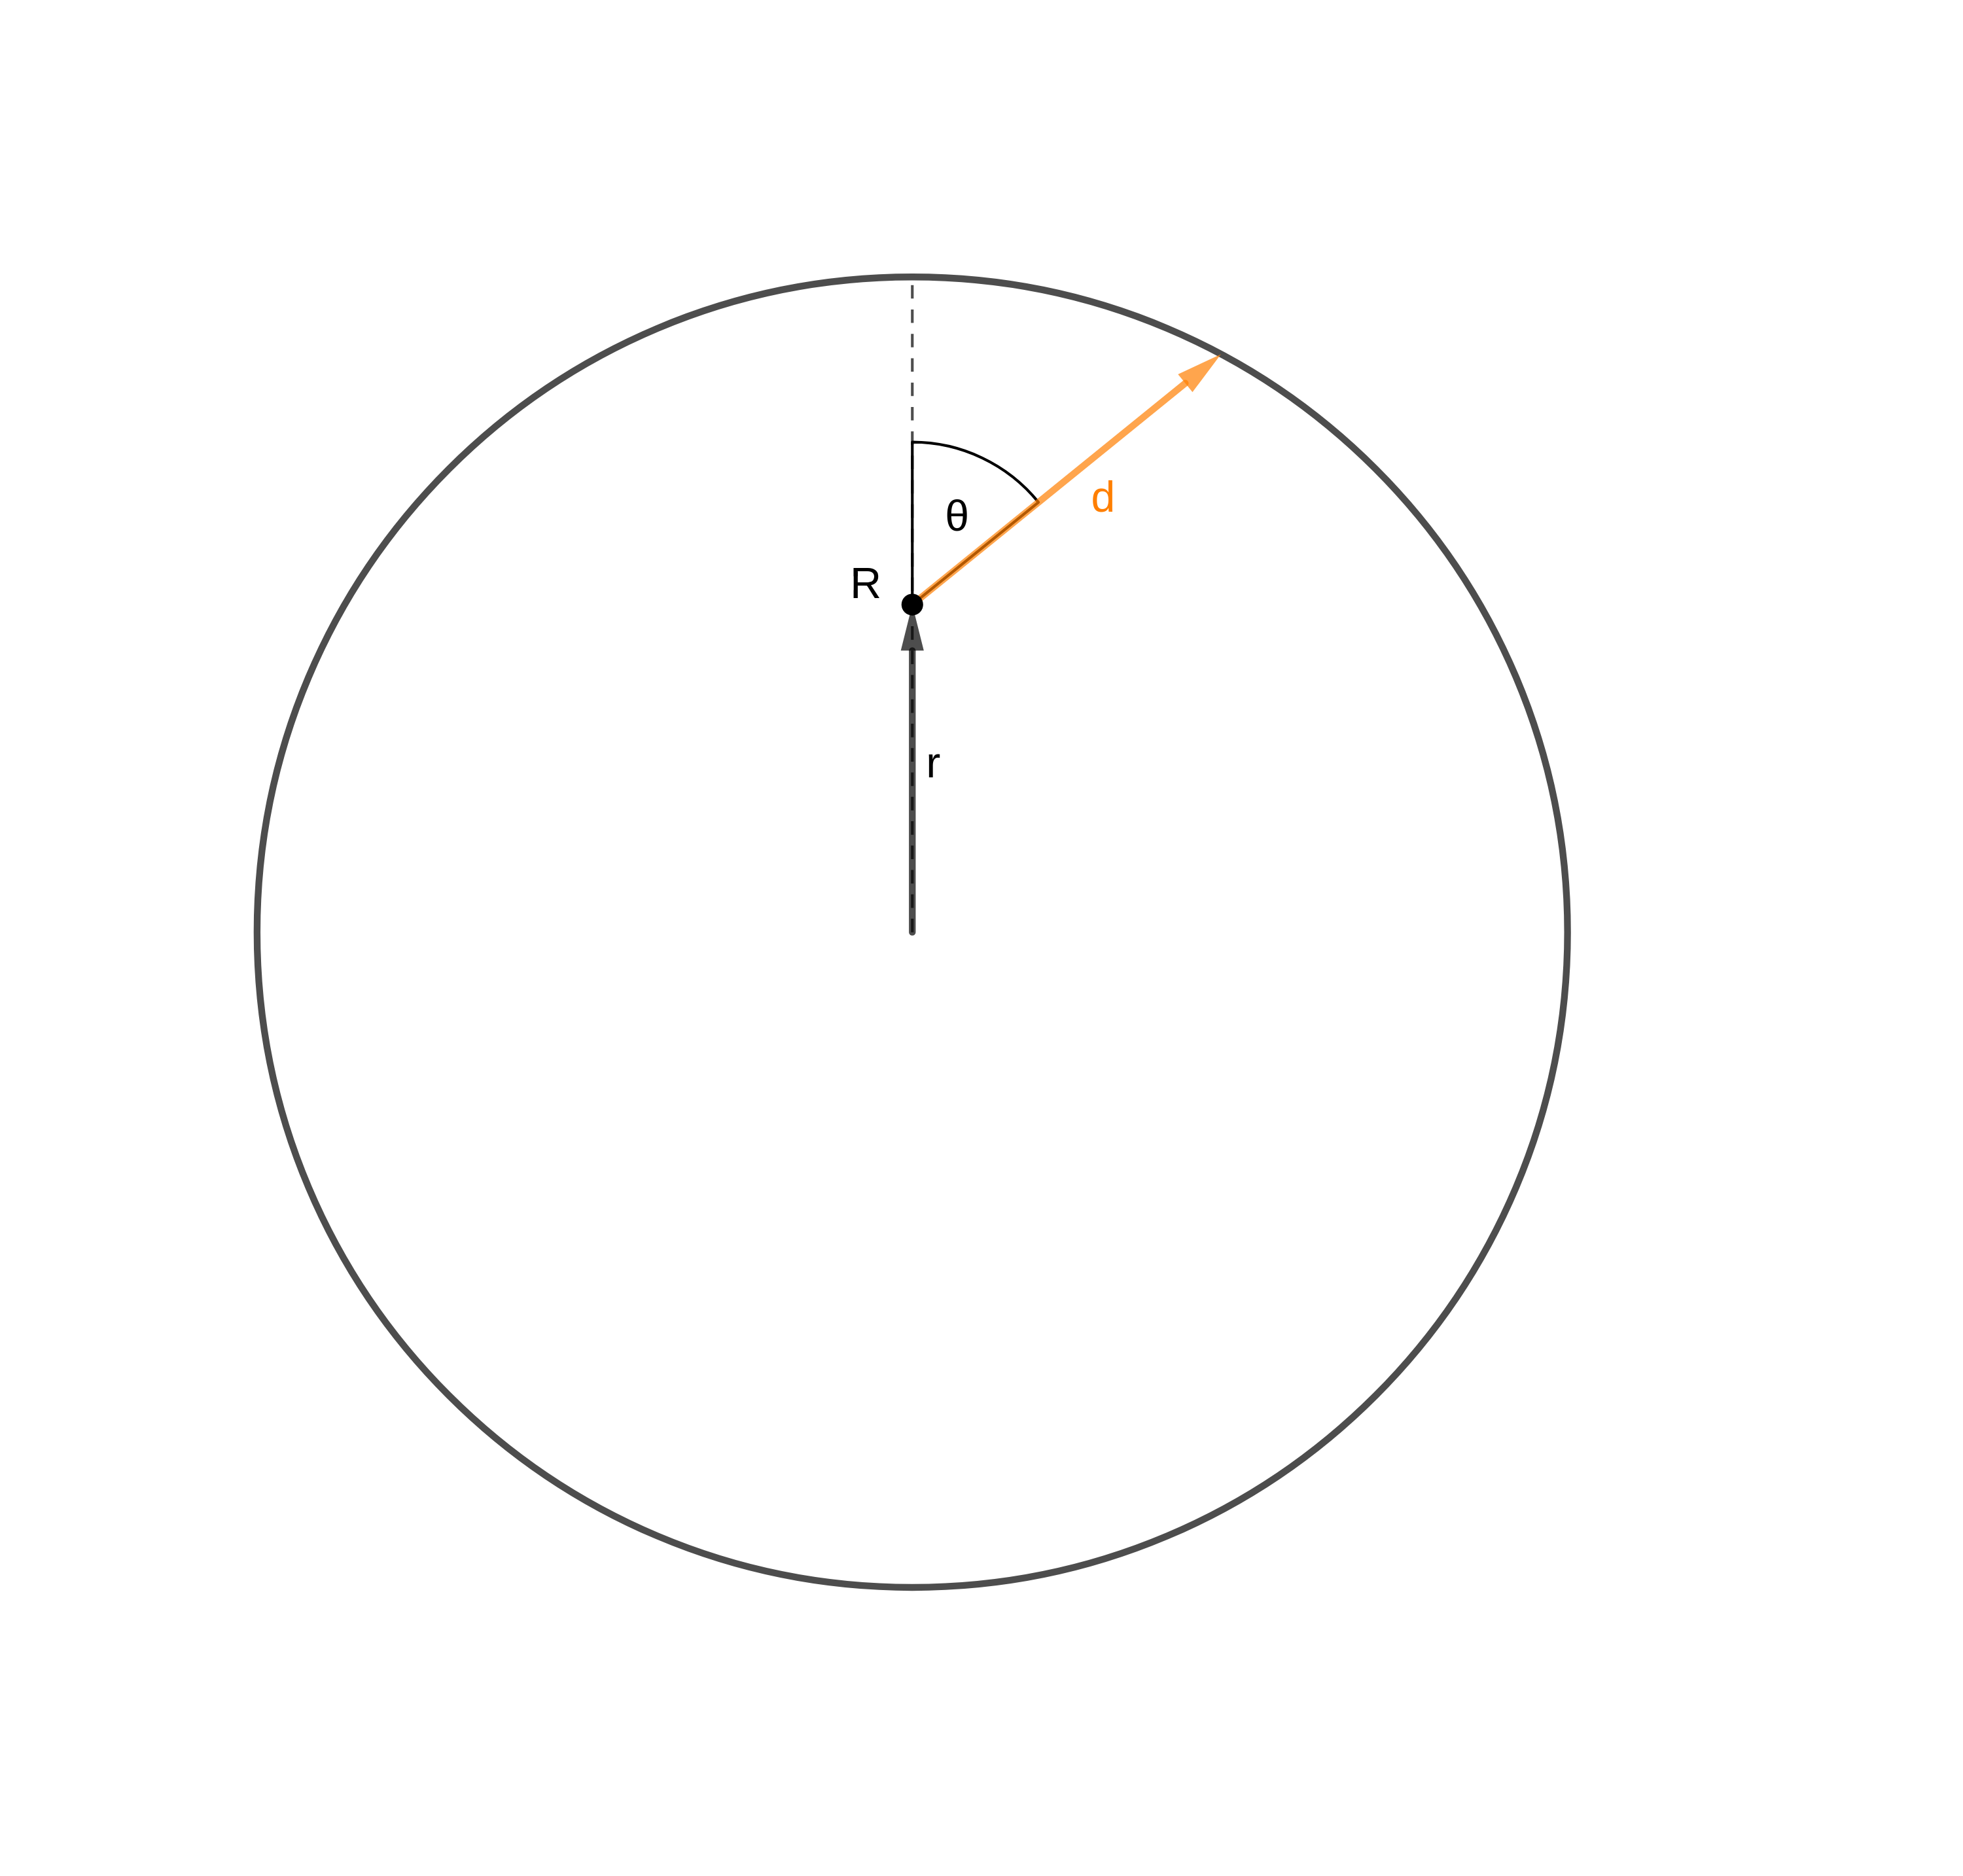
\includegraphics[width=.60\linewidth]{pobeg} 
    \caption{Pobeg žarka gama iz sfere z~radijem $R$.}
    \label{slika4} 
\end{figure}
Pri reševanju bomo naključno žrebali dolžine poti $d$ (oziroma njihovo lokacijo in smer
v~krogli), ki jo žarek mora prepotovati, da uide iz krogle, kar preko kosinusnega 
izreka zapišemo kot:
\begin{equation}
    d = -r\cos\theta + \sqrt{R^2 - r^2 \sin^2 \theta}
\end{equation}
kjer $r$ in $\theta$ generiramo na že znan način: 
\begin{align}
    r &= \sqrt[3]{u}, \\
    \theta &= \arccos(2v-1),
\end{align}
kjer sta $u, \, v$ uniformno porazdeljena na intervalu $[0,R]$ oziroma $[0,1]$.
Porazdelitev poti žarkov po poti, ki jo pa žarek dejansko prepotuje preden se sipa je podana
s~funkcijo:
\begin{equation}
    \frac{\text{d}P}{\text{d}s} = f(s) = \frac{1}{\mu} \mathrm{e}^{-s/\mu}
\end{equation}
kjer je parameter $\mu$ absorpcijska dolžina. To lahko obrnemo, da dobimo ven enačbo
po kateri moramo generirati dolžino poti:
\begin{equation}
    \frac{\text{d}P}{\text{d}t} = \frac{\text{d}P}{\text{d}s} \frac{\text{d}s}{\text{d}t} =
    \frac{1}{\mu} \mathrm{e}^{-s/\mu} \frac{\text{d}s}{\text{d}t} = 1
\end{equation}
kar pointegriramo in dobimo
\begin{equation}
    t = 1 - \mathrm{e}^{-s/\mu} \quad \rightarrow \quad s = - \ln (1-t)
\end{equation}
kjer je $t$ enakomerno izžrebana z~intervala $[0,1]$.\\
Pri računanju zdaj na vsakem koraku generiramo pot $d$, preverimo, če je manjša od $s$ 
(če bo žarek ušel iz krogle preden se bo sipal) in preštejemo vse žarke, ki so
ustrezali temu pogoju. Iz takega računanja bomo ven dobili verjetnost za pobeg
v~odvisnosti od razmerja med $\alpha = R/\mu$. Za to razmerje lahko že iz zapisa vidimo,
da ko bo radij veliko večji od proste poti šlo proti nič in obratno za veliko manjše
radij šlo razmerje proti ena. To lahko potrdimo tudi z~grafom~\ref{slika5}. Na 
grafu~\ref{slika6} zraven tudi vidimo, kako se spreminja varianca z~naraščanjem
razmerja $\alpha$ in medtem ko zgleda, da ima absolutna napaka nek maksimum, relativna
napaka ves čas korensko pada.
\begin{figure}    
    \centering
    \resizebox{0.75\linewidth}{!}{% GNUPLOT: LaTeX picture with Postscript
\begingroup
  \makeatletter
  \providecommand\color[2][]{%
    \GenericError{(gnuplot) \space\space\space\@spaces}{%
      Package color not loaded in conjunction with
      terminal option `colourtext'%
    }{See the gnuplot documentation for explanation.%
    }{Either use 'blacktext' in gnuplot or load the package
      color.sty in LaTeX.}%
    \renewcommand\color[2][]{}%
  }%
  \providecommand\includegraphics[2][]{%
    \GenericError{(gnuplot) \space\space\space\@spaces}{%
      Package graphicx or graphics not loaded%
    }{See the gnuplot documentation for explanation.%
    }{The gnuplot epslatex terminal needs graphicx.sty or graphics.sty.}%
    \renewcommand\includegraphics[2][]{}%
  }%
  \providecommand\rotatebox[2]{#2}%
  \@ifundefined{ifGPcolor}{%
    \newif\ifGPcolor
    \GPcolortrue
  }{}%
  \@ifundefined{ifGPblacktext}{%
    \newif\ifGPblacktext
    \GPblacktexttrue
  }{}%
  % define a \g@addto@macro without @ in the name:
  \let\gplgaddtomacro\g@addto@macro
  % define empty templates for all commands taking text:
  \gdef\gplbacktext{}%
  \gdef\gplfronttext{}%
  \makeatother
  \ifGPblacktext
    % no textcolor at all
    \def\colorrgb#1{}%
    \def\colorgray#1{}%
  \else
    % gray or color?
    \ifGPcolor
      \def\colorrgb#1{\color[rgb]{#1}}%
      \def\colorgray#1{\color[gray]{#1}}%
      \expandafter\def\csname LTw\endcsname{\color{white}}%
      \expandafter\def\csname LTb\endcsname{\color{black}}%
      \expandafter\def\csname LTa\endcsname{\color{black}}%
      \expandafter\def\csname LT0\endcsname{\color[rgb]{1,0,0}}%
      \expandafter\def\csname LT1\endcsname{\color[rgb]{0,1,0}}%
      \expandafter\def\csname LT2\endcsname{\color[rgb]{0,0,1}}%
      \expandafter\def\csname LT3\endcsname{\color[rgb]{1,0,1}}%
      \expandafter\def\csname LT4\endcsname{\color[rgb]{0,1,1}}%
      \expandafter\def\csname LT5\endcsname{\color[rgb]{1,1,0}}%
      \expandafter\def\csname LT6\endcsname{\color[rgb]{0,0,0}}%
      \expandafter\def\csname LT7\endcsname{\color[rgb]{1,0.3,0}}%
      \expandafter\def\csname LT8\endcsname{\color[rgb]{0.5,0.5,0.5}}%
    \else
      % gray
      \def\colorrgb#1{\color{black}}%
      \def\colorgray#1{\color[gray]{#1}}%
      \expandafter\def\csname LTw\endcsname{\color{white}}%
      \expandafter\def\csname LTb\endcsname{\color{black}}%
      \expandafter\def\csname LTa\endcsname{\color{black}}%
      \expandafter\def\csname LT0\endcsname{\color{black}}%
      \expandafter\def\csname LT1\endcsname{\color{black}}%
      \expandafter\def\csname LT2\endcsname{\color{black}}%
      \expandafter\def\csname LT3\endcsname{\color{black}}%
      \expandafter\def\csname LT4\endcsname{\color{black}}%
      \expandafter\def\csname LT5\endcsname{\color{black}}%
      \expandafter\def\csname LT6\endcsname{\color{black}}%
      \expandafter\def\csname LT7\endcsname{\color{black}}%
      \expandafter\def\csname LT8\endcsname{\color{black}}%
    \fi
  \fi
    \setlength{\unitlength}{0.0500bp}%
    \ifx\gptboxheight\undefined%
      \newlength{\gptboxheight}%
      \newlength{\gptboxwidth}%
      \newsavebox{\gptboxtext}%
    \fi%
    \setlength{\fboxrule}{0.5pt}%
    \setlength{\fboxsep}{1pt}%
\begin{picture}(7200.00,5040.00)%
    \gplgaddtomacro\gplbacktext{%
      \csname LTb\endcsname%%
      \put(594,220){\makebox(0,0)[r]{\strut{}$-18$}}%
      \csname LTb\endcsname%%
      \put(594,950){\makebox(0,0)[r]{\strut{}$-15$}}%
      \csname LTb\endcsname%%
      \put(594,1680){\makebox(0,0)[r]{\strut{}$-12$}}%
      \csname LTb\endcsname%%
      \put(594,2410){\makebox(0,0)[r]{\strut{}$-9$}}%
      \csname LTb\endcsname%%
      \put(594,3139){\makebox(0,0)[r]{\strut{}$-6$}}%
      \csname LTb\endcsname%%
      \put(594,3869){\makebox(0,0)[r]{\strut{}$-3$}}%
      \csname LTb\endcsname%%
      \put(594,4599){\makebox(0,0)[r]{\strut{}$0$}}%
      \csname LTb\endcsname%%
      \put(726,0){\makebox(0,0){\strut{}}}%
      \csname LTb\endcsname%%
      \put(2245,0){\makebox(0,0){\strut{}}}%
      \csname LTb\endcsname%%
      \put(3765,0){\makebox(0,0){\strut{}}}%
      \csname LTb\endcsname%%
      \put(5284,0){\makebox(0,0){\strut{}}}%
      \csname LTb\endcsname%%
      \put(6803,0){\makebox(0,0){\strut{}}}%
      \put(726,4819){\makebox(0,0){\strut{}$0$}}%
      \put(2245,4819){\makebox(0,0){\strut{}$4$}}%
      \put(3765,4819){\makebox(0,0){\strut{}$8$}}%
      \put(5284,4819){\makebox(0,0){\strut{}$12$}}%
      \put(6803,4819){\makebox(0,0){\strut{}$16$}}%
    }%
    \gplgaddtomacro\gplfronttext{%
      \csname LTb\endcsname%%
      \put(3764,4426){\makebox(0,0){\strut{}sosedi}}%
      \csname LTb\endcsname%%
      \put(3334,3084){\makebox(0,0)[l]{\strut{}$T = 0 $}}%
      \csname LTb\endcsname%%
      \put(3334,3304){\makebox(0,0)[l]{\strut{}$T = 0.1 $}}%
      \csname LTb\endcsname%%
      \put(3334,3524){\makebox(0,0)[l]{\strut{}$T = 0.25 $}}%
      \csname LTb\endcsname%%
      \put(3334,3744){\makebox(0,0)[l]{\strut{}$T = 0.5 $}}%
      \csname LTb\endcsname%%
      \put(3334,3964){\makebox(0,0)[l]{\strut{}$T = 1 $}}%
      \csname LTb\endcsname%%
      \put(3334,4184){\makebox(0,0)[l]{\strut{}$T = 5 $}}%
    }%
    \gplbacktext
    \put(0,0){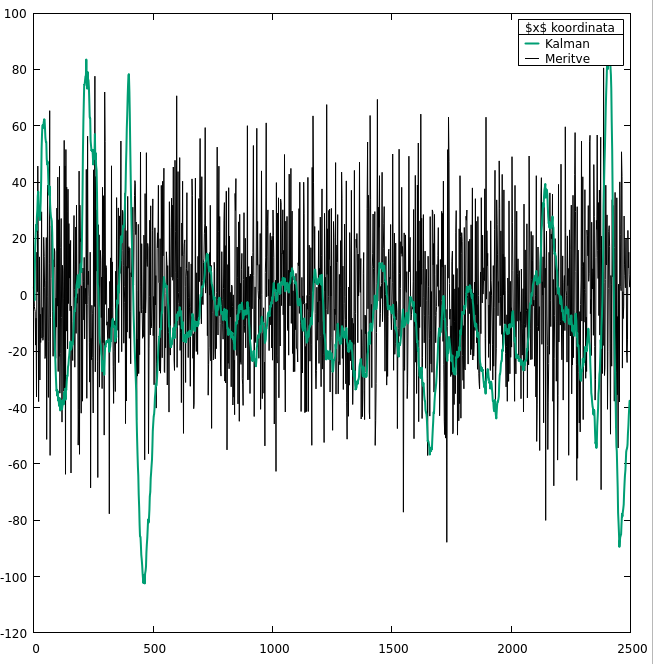
\includegraphics{graf5}}%
    \gplfronttext
  \end{picture}%
\endgroup
}
    \caption{Spreminjanje verjetnosti za pobeg z~večanjem razmerja $\mu/R$.}
    \label{slika5}
\end{figure}
\begin{figure}    
    \centering
    \resizebox{0.75\linewidth}{!}{% GNUPLOT: LaTeX picture with Postscript
\begingroup
  \makeatletter
  \providecommand\color[2][]{%
    \GenericError{(gnuplot) \space\space\space\@spaces}{%
      Package color not loaded in conjunction with
      terminal option `colourtext'%
    }{See the gnuplot documentation for explanation.%
    }{Either use 'blacktext' in gnuplot or load the package
      color.sty in LaTeX.}%
    \renewcommand\color[2][]{}%
  }%
  \providecommand\includegraphics[2][]{%
    \GenericError{(gnuplot) \space\space\space\@spaces}{%
      Package graphicx or graphics not loaded%
    }{See the gnuplot documentation for explanation.%
    }{The gnuplot epslatex terminal needs graphicx.sty or graphics.sty.}%
    \renewcommand\includegraphics[2][]{}%
  }%
  \providecommand\rotatebox[2]{#2}%
  \@ifundefined{ifGPcolor}{%
    \newif\ifGPcolor
    \GPcolortrue
  }{}%
  \@ifundefined{ifGPblacktext}{%
    \newif\ifGPblacktext
    \GPblacktexttrue
  }{}%
  % define a \g@addto@macro without @ in the name:
  \let\gplgaddtomacro\g@addto@macro
  % define empty templates for all commands taking text:
  \gdef\gplbacktext{}%
  \gdef\gplfronttext{}%
  \makeatother
  \ifGPblacktext
    % no textcolor at all
    \def\colorrgb#1{}%
    \def\colorgray#1{}%
  \else
    % gray or color?
    \ifGPcolor
      \def\colorrgb#1{\color[rgb]{#1}}%
      \def\colorgray#1{\color[gray]{#1}}%
      \expandafter\def\csname LTw\endcsname{\color{white}}%
      \expandafter\def\csname LTb\endcsname{\color{black}}%
      \expandafter\def\csname LTa\endcsname{\color{black}}%
      \expandafter\def\csname LT0\endcsname{\color[rgb]{1,0,0}}%
      \expandafter\def\csname LT1\endcsname{\color[rgb]{0,1,0}}%
      \expandafter\def\csname LT2\endcsname{\color[rgb]{0,0,1}}%
      \expandafter\def\csname LT3\endcsname{\color[rgb]{1,0,1}}%
      \expandafter\def\csname LT4\endcsname{\color[rgb]{0,1,1}}%
      \expandafter\def\csname LT5\endcsname{\color[rgb]{1,1,0}}%
      \expandafter\def\csname LT6\endcsname{\color[rgb]{0,0,0}}%
      \expandafter\def\csname LT7\endcsname{\color[rgb]{1,0.3,0}}%
      \expandafter\def\csname LT8\endcsname{\color[rgb]{0.5,0.5,0.5}}%
    \else
      % gray
      \def\colorrgb#1{\color{black}}%
      \def\colorgray#1{\color[gray]{#1}}%
      \expandafter\def\csname LTw\endcsname{\color{white}}%
      \expandafter\def\csname LTb\endcsname{\color{black}}%
      \expandafter\def\csname LTa\endcsname{\color{black}}%
      \expandafter\def\csname LT0\endcsname{\color{black}}%
      \expandafter\def\csname LT1\endcsname{\color{black}}%
      \expandafter\def\csname LT2\endcsname{\color{black}}%
      \expandafter\def\csname LT3\endcsname{\color{black}}%
      \expandafter\def\csname LT4\endcsname{\color{black}}%
      \expandafter\def\csname LT5\endcsname{\color{black}}%
      \expandafter\def\csname LT6\endcsname{\color{black}}%
      \expandafter\def\csname LT7\endcsname{\color{black}}%
      \expandafter\def\csname LT8\endcsname{\color{black}}%
    \fi
  \fi
    \setlength{\unitlength}{0.0500bp}%
    \ifx\gptboxheight\undefined%
      \newlength{\gptboxheight}%
      \newlength{\gptboxwidth}%
      \newsavebox{\gptboxtext}%
    \fi%
    \setlength{\fboxrule}{0.5pt}%
    \setlength{\fboxsep}{1pt}%
\begin{picture}(7200.00,5040.00)%
    \gplgaddtomacro\gplbacktext{%
      \csname LTb\endcsname%%
      \put(462,440){\makebox(0,0)[r]{\strut{}$0$}}%
      \put(462,1316){\makebox(0,0)[r]{\strut{}$5$}}%
      \put(462,2192){\makebox(0,0)[r]{\strut{}$10$}}%
      \put(462,3067){\makebox(0,0)[r]{\strut{}$15$}}%
      \put(462,3943){\makebox(0,0)[r]{\strut{}$20$}}%
      \put(462,4819){\makebox(0,0)[r]{\strut{}$25$}}%
      \put(594,220){\makebox(0,0){\strut{}$0$}}%
      \put(1836,220){\makebox(0,0){\strut{}$2$}}%
      \put(3078,220){\makebox(0,0){\strut{}$4$}}%
      \put(4319,220){\makebox(0,0){\strut{}$6$}}%
      \put(5561,220){\makebox(0,0){\strut{}$8$}}%
      \put(6803,220){\makebox(0,0){\strut{}$10$}}%
    }%
    \gplgaddtomacro\gplfronttext{%
      \csname LTb\endcsname%%
      \put(5086,3216){\makebox(0,0)[l]{\strut{}$ \Delta t = 0.001$}}%
      \csname LTb\endcsname%%
      \put(5086,3436){\makebox(0,0)[l]{\strut{}$ \Delta t = 0.01$}}%
      \csname LTb\endcsname%%
      \put(5086,3656){\makebox(0,0)[l]{\strut{}$ \Delta t = 0.1$}}%
      \csname LTb\endcsname%%
      \put(5086,3876){\makebox(0,0)[l]{\strut{}$ \Delta t = 0.25$}}%
      \csname LTb\endcsname%%
      \put(5086,4096){\makebox(0,0)[l]{\strut{}$ \Delta t = 0.5$}}%
      \csname LTb\endcsname%%
      \put(5086,4316){\makebox(0,0)[l]{\strut{}$ \Delta t = 1$}}%
      \csname LTb\endcsname%%
      \put(5086,4536){\makebox(0,0)[l]{\strut{}$N_0 \mathrm{e}^{-\beta t}$}}%
    }%
    \gplbacktext
    \put(0,0){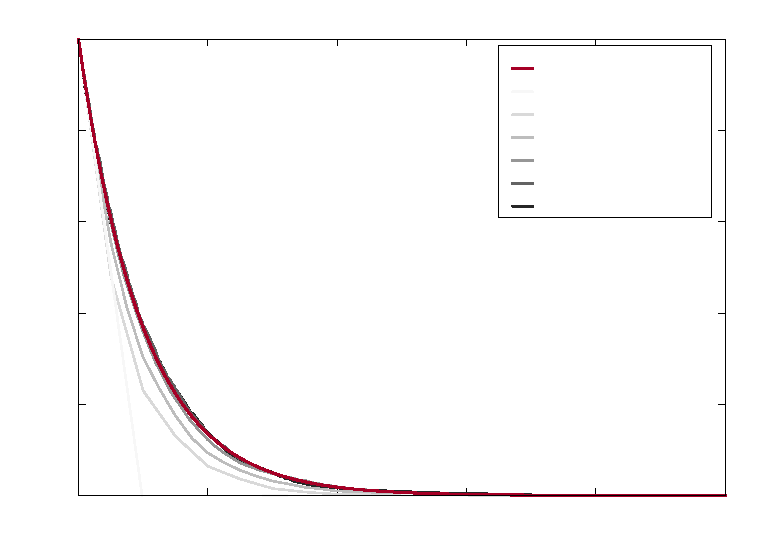
\includegraphics[width={360.00bp},height={252.00bp}]{graf6}}%
    \gplfronttext
  \end{picture}%
\endgroup
}
    \caption{Spreminjanje absolutne oziroma relativne napake verjetnosti za pobeg.}
    \label{slika6}
\end{figure}
\pagebreak

%----------------------------------------------------------------------------------------
%	PROBLEM 3
%----------------------------------------------------------------------------------------
\section{Prepustna plošča}

\begin{figure}
    \centering 
    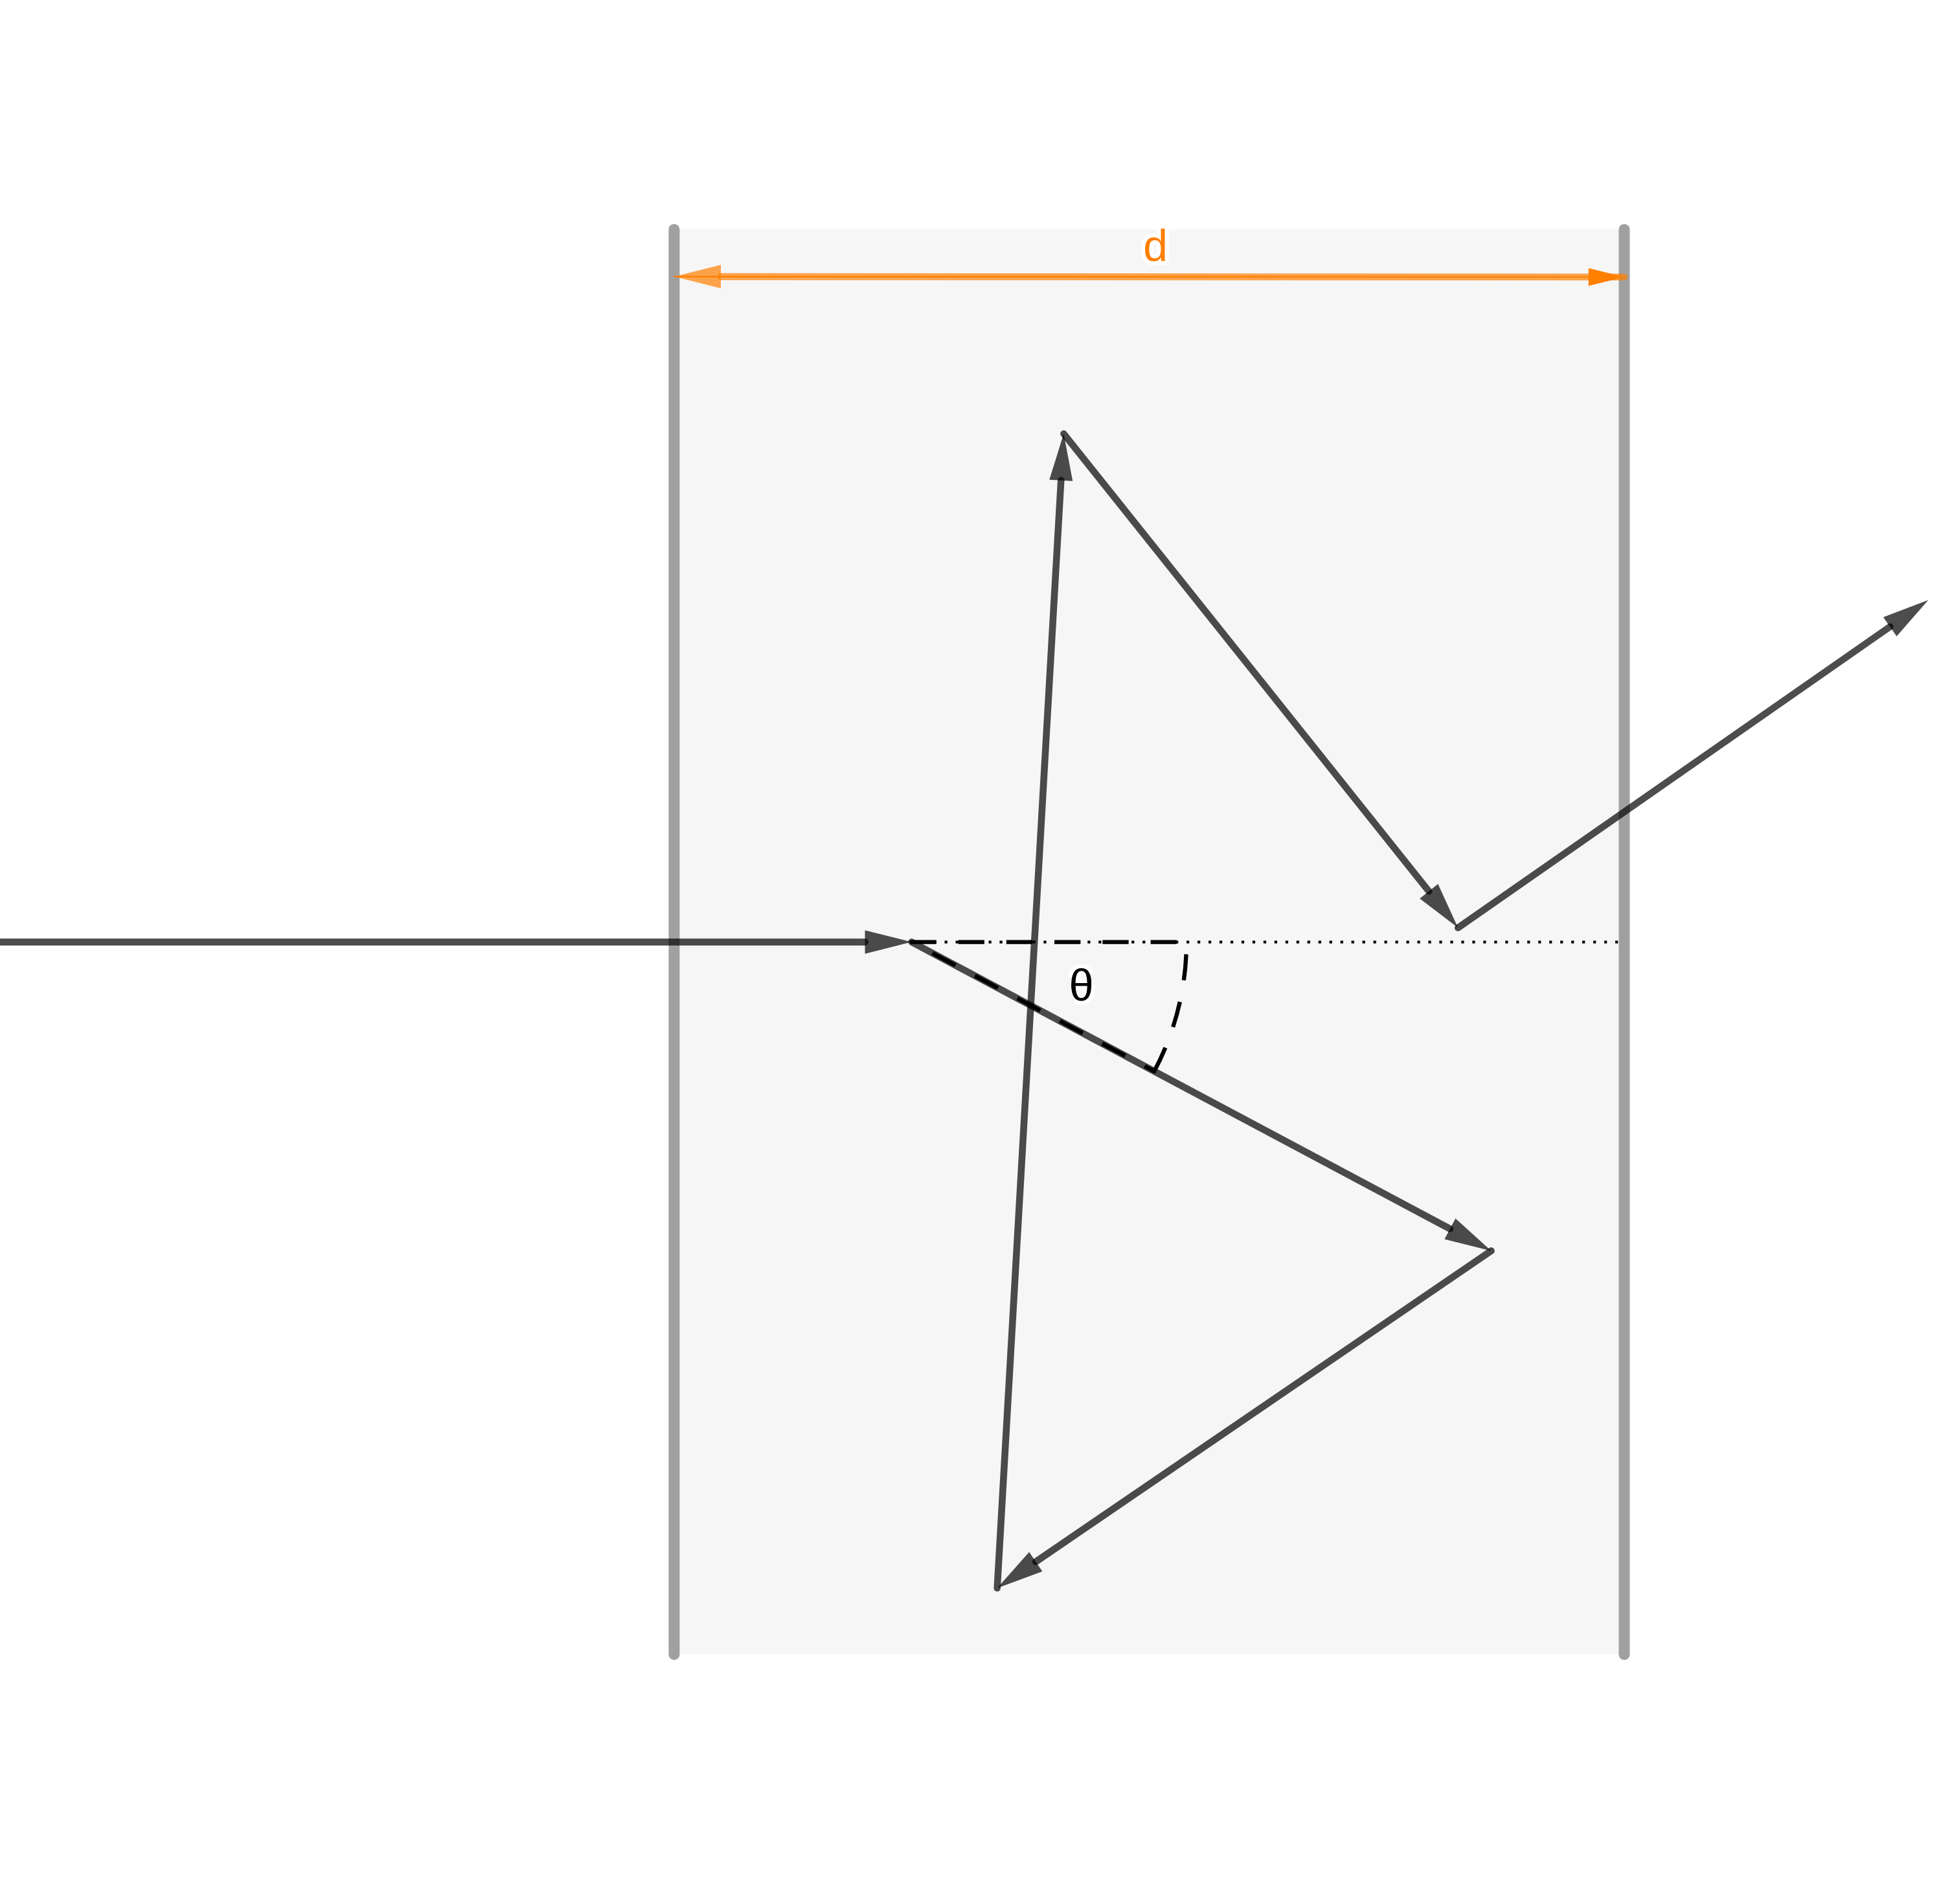
\includegraphics[width=.60\linewidth]{sipanje} 
    \caption{Pot žarka nevtronov skozi ploščo debeline $d$.}
    \label{slika7} 
\end{figure}
Tok nevtronov vpada pravokotno na ploščo v~kateri se nevtroni sipajo, njihova povprečna
dolžina $\mu$ pa je enaka polovici razdalje med ploščama $d$. Primer poteka potovanja
enega žarka skozi tako ploščo je prikazan na sliki~\ref{slika7}.
Omejimo se na različna primera:
\begin{itemize}
    \item nevtron se lahko sipa le naprej/nazaj (enodimenzionalen problem),
    \item nevtron se lahko sipa poljubno v~vse smeri.
\end{itemize}
Zanima nas odbojnost oziroma prepustnost take plošče in kolikokrat se žarek siplje na taki
poti.
\subsubsection*{1D}
Enako kot pri prejšnji nalogi imamo generator poti $s$, ki ga delec opravi preden se siplje
\begin{equation}
    s = - \ln (1-t),
\end{equation}
kjer je $t$ enakomerno izžrebana z~intervala $[0,1]$. Žarku sledimo ob vsakem sipanju
in njegovo celotno pot izračunamo na slednji način:
\begin{equation}
    x_{i+1} = x_i \pm s_i.
\end{equation}
Ali bo $+$ ali $-$ določimo z~naključnim celim številom $n$: $ \pm = 2 (n\%2) - 1$.
Za vsake žarek si shranjujemo koliko trkov je prestal v~plošči in ali je šel ven skozi
isto ploščo kot je prišel noter ali na nasprotni strani, iz česar bomo izračunali
prepustnost in odbojnost.

\subsubsection*{3D}
Zdaj moramo spet preiti na sferične koordinate, ki jih generiramo na že večkrat uporabljen
način (namesto $r$ zdaj vzamemo $s$):
\begin{align}
    \phi &= 2 \pi u, \\
    \theta &= \arccos(2v-1), \\
    s &= - \ln (1-t).
\end{align}
Podobno opazujemo posamezen žarek:
\begin{equation}
    x_{i+1} = x_i + s_i \sin\theta_i \cos\phi_i.
\end{equation}

\subsection{Rezultati}
Dobljena prepustnost in odbojnost sta predstavljena v~naslednji tabeli:

\begin{tabularx}{\textwidth}{ |c|X|X| }
    \hline
    \quad & $T$ & $R$ \\
    \hline
    1D & $0,494302 \pm 10^{-6}$  & $0,505698 \pm 10^{-6}$ \\
    \hline
    3D & $0,482966 \pm 10^{-6}$  & $0,517034 \pm 10^{-6}$ \\
    \hline
\end{tabularx}

Vidimo, da sta rezultata precej podobna, razlika pa verjetno izhaja iz preveč 
poenostavljenega problema v~eni dimenziji. Na grafu~\ref{slika8} lahko tudi vidimo, da 
je pri obeh procesih število trkov enako porazdeljeno.
\begin{figure}    
    \centering
    \resizebox{0.75\linewidth}{!}{% GNUPLOT: LaTeX picture with Postscript
\begingroup
  \makeatletter
  \providecommand\color[2][]{%
    \GenericError{(gnuplot) \space\space\space\@spaces}{%
      Package color not loaded in conjunction with
      terminal option `colourtext'%
    }{See the gnuplot documentation for explanation.%
    }{Either use 'blacktext' in gnuplot or load the package
      color.sty in LaTeX.}%
    \renewcommand\color[2][]{}%
  }%
  \providecommand\includegraphics[2][]{%
    \GenericError{(gnuplot) \space\space\space\@spaces}{%
      Package graphicx or graphics not loaded%
    }{See the gnuplot documentation for explanation.%
    }{The gnuplot epslatex terminal needs graphicx.sty or graphics.sty.}%
    \renewcommand\includegraphics[2][]{}%
  }%
  \providecommand\rotatebox[2]{#2}%
  \@ifundefined{ifGPcolor}{%
    \newif\ifGPcolor
    \GPcolortrue
  }{}%
  \@ifundefined{ifGPblacktext}{%
    \newif\ifGPblacktext
    \GPblacktexttrue
  }{}%
  % define a \g@addto@macro without @ in the name:
  \let\gplgaddtomacro\g@addto@macro
  % define empty templates for all commands taking text:
  \gdef\gplbacktext{}%
  \gdef\gplfronttext{}%
  \makeatother
  \ifGPblacktext
    % no textcolor at all
    \def\colorrgb#1{}%
    \def\colorgray#1{}%
  \else
    % gray or color?
    \ifGPcolor
      \def\colorrgb#1{\color[rgb]{#1}}%
      \def\colorgray#1{\color[gray]{#1}}%
      \expandafter\def\csname LTw\endcsname{\color{white}}%
      \expandafter\def\csname LTb\endcsname{\color{black}}%
      \expandafter\def\csname LTa\endcsname{\color{black}}%
      \expandafter\def\csname LT0\endcsname{\color[rgb]{1,0,0}}%
      \expandafter\def\csname LT1\endcsname{\color[rgb]{0,1,0}}%
      \expandafter\def\csname LT2\endcsname{\color[rgb]{0,0,1}}%
      \expandafter\def\csname LT3\endcsname{\color[rgb]{1,0,1}}%
      \expandafter\def\csname LT4\endcsname{\color[rgb]{0,1,1}}%
      \expandafter\def\csname LT5\endcsname{\color[rgb]{1,1,0}}%
      \expandafter\def\csname LT6\endcsname{\color[rgb]{0,0,0}}%
      \expandafter\def\csname LT7\endcsname{\color[rgb]{1,0.3,0}}%
      \expandafter\def\csname LT8\endcsname{\color[rgb]{0.5,0.5,0.5}}%
    \else
      % gray
      \def\colorrgb#1{\color{black}}%
      \def\colorgray#1{\color[gray]{#1}}%
      \expandafter\def\csname LTw\endcsname{\color{white}}%
      \expandafter\def\csname LTb\endcsname{\color{black}}%
      \expandafter\def\csname LTa\endcsname{\color{black}}%
      \expandafter\def\csname LT0\endcsname{\color{black}}%
      \expandafter\def\csname LT1\endcsname{\color{black}}%
      \expandafter\def\csname LT2\endcsname{\color{black}}%
      \expandafter\def\csname LT3\endcsname{\color{black}}%
      \expandafter\def\csname LT4\endcsname{\color{black}}%
      \expandafter\def\csname LT5\endcsname{\color{black}}%
      \expandafter\def\csname LT6\endcsname{\color{black}}%
      \expandafter\def\csname LT7\endcsname{\color{black}}%
      \expandafter\def\csname LT8\endcsname{\color{black}}%
    \fi
  \fi
    \setlength{\unitlength}{0.0500bp}%
    \ifx\gptboxheight\undefined%
      \newlength{\gptboxheight}%
      \newlength{\gptboxwidth}%
      \newsavebox{\gptboxtext}%
    \fi%
    \setlength{\fboxrule}{0.5pt}%
    \setlength{\fboxsep}{1pt}%
\begin{picture}(7200.00,5040.00)%
    \gplgaddtomacro\gplbacktext{%
      \csname LTb\endcsname%%
      \put(594,220){\makebox(0,0)[r]{\strut{}$-18$}}%
      \csname LTb\endcsname%%
      \put(594,950){\makebox(0,0)[r]{\strut{}$-15$}}%
      \csname LTb\endcsname%%
      \put(594,1680){\makebox(0,0)[r]{\strut{}$-12$}}%
      \csname LTb\endcsname%%
      \put(594,2410){\makebox(0,0)[r]{\strut{}$-9$}}%
      \csname LTb\endcsname%%
      \put(594,3139){\makebox(0,0)[r]{\strut{}$-6$}}%
      \csname LTb\endcsname%%
      \put(594,3869){\makebox(0,0)[r]{\strut{}$-3$}}%
      \csname LTb\endcsname%%
      \put(594,4599){\makebox(0,0)[r]{\strut{}$0$}}%
      \csname LTb\endcsname%%
      \put(726,0){\makebox(0,0){\strut{}}}%
      \csname LTb\endcsname%%
      \put(2245,0){\makebox(0,0){\strut{}}}%
      \csname LTb\endcsname%%
      \put(3765,0){\makebox(0,0){\strut{}}}%
      \csname LTb\endcsname%%
      \put(5284,0){\makebox(0,0){\strut{}}}%
      \csname LTb\endcsname%%
      \put(6803,0){\makebox(0,0){\strut{}}}%
      \put(726,4819){\makebox(0,0){\strut{}$0$}}%
      \put(2245,4819){\makebox(0,0){\strut{}$4$}}%
      \put(3765,4819){\makebox(0,0){\strut{}$8$}}%
      \put(5284,4819){\makebox(0,0){\strut{}$12$}}%
      \put(6803,4819){\makebox(0,0){\strut{}$16$}}%
    }%
    \gplgaddtomacro\gplfronttext{%
      \csname LTb\endcsname%%
      \put(3764,4426){\makebox(0,0){\strut{}poljubni}}%
      \csname LTb\endcsname%%
      \put(3334,3084){\makebox(0,0)[l]{\strut{}$T = 0 $}}%
      \csname LTb\endcsname%%
      \put(3334,3304){\makebox(0,0)[l]{\strut{}$T = 0.1 $}}%
      \csname LTb\endcsname%%
      \put(3334,3524){\makebox(0,0)[l]{\strut{}$T = 0.25 $}}%
      \csname LTb\endcsname%%
      \put(3334,3744){\makebox(0,0)[l]{\strut{}$T = 0.5 $}}%
      \csname LTb\endcsname%%
      \put(3334,3964){\makebox(0,0)[l]{\strut{}$T = 1 $}}%
      \csname LTb\endcsname%%
      \put(3334,4184){\makebox(0,0)[l]{\strut{}$T = 5 $}}%
    }%
    \gplbacktext
    \put(0,0){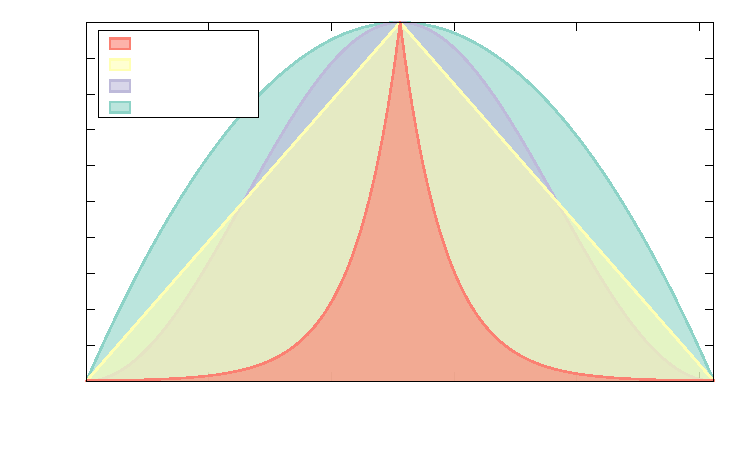
\includegraphics{graf4}}%
    \gplfronttext
  \end{picture}%
\endgroup
}
    \caption{Porazdelitev po številu sipanj za oba primera.}
    \label{slika8}
\end{figure}
Nazadnje si lahko še pogledamo, kako se prepustnost žarkov spreminja z~debelino stene
(tako kot v prejšnji nalogi spreminjamo razmerje $\alpha = \mu/d$). Z~grafa~\ref{slika9}
lahko vidimo, da ta odvisnost eksponentno raste, razlika med različnima metodama izračuna
pa je zanemarljivo majhna. Na histogramu~\ref{slika10} vidimo kako z~večanjem razmerja
$\alpha$, se pravi z~manjšanjem debeline plošče, števila trkov za posamezen žarek 
dobiva bolj izrazit maksimum pri dveh/treh trkih in jih veliko več preleti ploščo,
ne da bi se sipali, kar tudi pojasni obliko grafa~\ref{slika9}.\\
\begin{figure}    
    \centering
    \resizebox{0.75\linewidth}{!}{% GNUPLOT: LaTeX picture with Postscript
\begingroup
  \makeatletter
  \providecommand\color[2][]{%
    \GenericError{(gnuplot) \space\space\space\@spaces}{%
      Package color not loaded in conjunction with
      terminal option `colourtext'%
    }{See the gnuplot documentation for explanation.%
    }{Either use 'blacktext' in gnuplot or load the package
      color.sty in LaTeX.}%
    \renewcommand\color[2][]{}%
  }%
  \providecommand\includegraphics[2][]{%
    \GenericError{(gnuplot) \space\space\space\@spaces}{%
      Package graphicx or graphics not loaded%
    }{See the gnuplot documentation for explanation.%
    }{The gnuplot epslatex terminal needs graphicx.sty or graphics.sty.}%
    \renewcommand\includegraphics[2][]{}%
  }%
  \providecommand\rotatebox[2]{#2}%
  \@ifundefined{ifGPcolor}{%
    \newif\ifGPcolor
    \GPcolortrue
  }{}%
  \@ifundefined{ifGPblacktext}{%
    \newif\ifGPblacktext
    \GPblacktexttrue
  }{}%
  % define a \g@addto@macro without @ in the name:
  \let\gplgaddtomacro\g@addto@macro
  % define empty templates for all commands taking text:
  \gdef\gplbacktext{}%
  \gdef\gplfronttext{}%
  \makeatother
  \ifGPblacktext
    % no textcolor at all
    \def\colorrgb#1{}%
    \def\colorgray#1{}%
  \else
    % gray or color?
    \ifGPcolor
      \def\colorrgb#1{\color[rgb]{#1}}%
      \def\colorgray#1{\color[gray]{#1}}%
      \expandafter\def\csname LTw\endcsname{\color{white}}%
      \expandafter\def\csname LTb\endcsname{\color{black}}%
      \expandafter\def\csname LTa\endcsname{\color{black}}%
      \expandafter\def\csname LT0\endcsname{\color[rgb]{1,0,0}}%
      \expandafter\def\csname LT1\endcsname{\color[rgb]{0,1,0}}%
      \expandafter\def\csname LT2\endcsname{\color[rgb]{0,0,1}}%
      \expandafter\def\csname LT3\endcsname{\color[rgb]{1,0,1}}%
      \expandafter\def\csname LT4\endcsname{\color[rgb]{0,1,1}}%
      \expandafter\def\csname LT5\endcsname{\color[rgb]{1,1,0}}%
      \expandafter\def\csname LT6\endcsname{\color[rgb]{0,0,0}}%
      \expandafter\def\csname LT7\endcsname{\color[rgb]{1,0.3,0}}%
      \expandafter\def\csname LT8\endcsname{\color[rgb]{0.5,0.5,0.5}}%
    \else
      % gray
      \def\colorrgb#1{\color{black}}%
      \def\colorgray#1{\color[gray]{#1}}%
      \expandafter\def\csname LTw\endcsname{\color{white}}%
      \expandafter\def\csname LTb\endcsname{\color{black}}%
      \expandafter\def\csname LTa\endcsname{\color{black}}%
      \expandafter\def\csname LT0\endcsname{\color{black}}%
      \expandafter\def\csname LT1\endcsname{\color{black}}%
      \expandafter\def\csname LT2\endcsname{\color{black}}%
      \expandafter\def\csname LT3\endcsname{\color{black}}%
      \expandafter\def\csname LT4\endcsname{\color{black}}%
      \expandafter\def\csname LT5\endcsname{\color{black}}%
      \expandafter\def\csname LT6\endcsname{\color{black}}%
      \expandafter\def\csname LT7\endcsname{\color{black}}%
      \expandafter\def\csname LT8\endcsname{\color{black}}%
    \fi
  \fi
    \setlength{\unitlength}{0.0500bp}%
    \ifx\gptboxheight\undefined%
      \newlength{\gptboxheight}%
      \newlength{\gptboxwidth}%
      \newsavebox{\gptboxtext}%
    \fi%
    \setlength{\fboxrule}{0.5pt}%
    \setlength{\fboxsep}{1pt}%
\begin{picture}(7200.00,5040.00)%
    \gplgaddtomacro\gplbacktext{%
      \csname LTb\endcsname%%
      \put(594,440){\makebox(0,0)[r]{\strut{}$0.1$}}%
      \put(594,1900){\makebox(0,0)[r]{\strut{}$1$}}%
      \put(594,3359){\makebox(0,0)[r]{\strut{}$10$}}%
      \put(594,4819){\makebox(0,0)[r]{\strut{}$100$}}%
      \put(726,220){\makebox(0,0){\strut{}$0$}}%
      \put(1941,220){\makebox(0,0){\strut{}$2$}}%
      \put(3157,220){\makebox(0,0){\strut{}$4$}}%
      \put(4372,220){\makebox(0,0){\strut{}$6$}}%
      \put(5588,220){\makebox(0,0){\strut{}$8$}}%
      \put(6803,220){\makebox(0,0){\strut{}$10$}}%
    }%
    \gplgaddtomacro\gplfronttext{%
      \csname LTb\endcsname%%
      \put(5086,3216){\makebox(0,0)[l]{\strut{}$ \Delta t = 0.001$}}%
      \csname LTb\endcsname%%
      \put(5086,3436){\makebox(0,0)[l]{\strut{}$ \Delta t = 0.01$}}%
      \csname LTb\endcsname%%
      \put(5086,3656){\makebox(0,0)[l]{\strut{}$ \Delta t = 0.1$}}%
      \csname LTb\endcsname%%
      \put(5086,3876){\makebox(0,0)[l]{\strut{}$ \Delta t = 0.25$}}%
      \csname LTb\endcsname%%
      \put(5086,4096){\makebox(0,0)[l]{\strut{}$ \Delta t = 0.5$}}%
      \csname LTb\endcsname%%
      \put(5086,4316){\makebox(0,0)[l]{\strut{}$ \Delta t = 1$}}%
      \csname LTb\endcsname%%
      \put(5086,4536){\makebox(0,0)[l]{\strut{}$N_0 \mathrm{e}^{-\beta t}$}}%
    }%
    \gplbacktext
    \put(0,0){\includegraphics[width={360.00bp},height={252.00bp}]{graf7}}%
    \gplfronttext
  \end{picture}%
\endgroup
}
    \caption{Spreminjanje prepustnosti in njene napake z~večanjem parametra $\alpha$.}
    \label{slika9}
\end{figure}
\begin{figure}    
    \centering
    \resizebox{0.75\linewidth}{!}{% GNUPLOT: LaTeX picture with Postscript
\begingroup
  \makeatletter
  \providecommand\color[2][]{%
    \GenericError{(gnuplot) \space\space\space\@spaces}{%
      Package color not loaded in conjunction with
      terminal option `colourtext'%
    }{See the gnuplot documentation for explanation.%
    }{Either use 'blacktext' in gnuplot or load the package
      color.sty in LaTeX.}%
    \renewcommand\color[2][]{}%
  }%
  \providecommand\includegraphics[2][]{%
    \GenericError{(gnuplot) \space\space\space\@spaces}{%
      Package graphicx or graphics not loaded%
    }{See the gnuplot documentation for explanation.%
    }{The gnuplot epslatex terminal needs graphicx.sty or graphics.sty.}%
    \renewcommand\includegraphics[2][]{}%
  }%
  \providecommand\rotatebox[2]{#2}%
  \@ifundefined{ifGPcolor}{%
    \newif\ifGPcolor
    \GPcolortrue
  }{}%
  \@ifundefined{ifGPblacktext}{%
    \newif\ifGPblacktext
    \GPblacktexttrue
  }{}%
  % define a \g@addto@macro without @ in the name:
  \let\gplgaddtomacro\g@addto@macro
  % define empty templates for all commands taking text:
  \gdef\gplbacktext{}%
  \gdef\gplfronttext{}%
  \makeatother
  \ifGPblacktext
    % no textcolor at all
    \def\colorrgb#1{}%
    \def\colorgray#1{}%
  \else
    % gray or color?
    \ifGPcolor
      \def\colorrgb#1{\color[rgb]{#1}}%
      \def\colorgray#1{\color[gray]{#1}}%
      \expandafter\def\csname LTw\endcsname{\color{white}}%
      \expandafter\def\csname LTb\endcsname{\color{black}}%
      \expandafter\def\csname LTa\endcsname{\color{black}}%
      \expandafter\def\csname LT0\endcsname{\color[rgb]{1,0,0}}%
      \expandafter\def\csname LT1\endcsname{\color[rgb]{0,1,0}}%
      \expandafter\def\csname LT2\endcsname{\color[rgb]{0,0,1}}%
      \expandafter\def\csname LT3\endcsname{\color[rgb]{1,0,1}}%
      \expandafter\def\csname LT4\endcsname{\color[rgb]{0,1,1}}%
      \expandafter\def\csname LT5\endcsname{\color[rgb]{1,1,0}}%
      \expandafter\def\csname LT6\endcsname{\color[rgb]{0,0,0}}%
      \expandafter\def\csname LT7\endcsname{\color[rgb]{1,0.3,0}}%
      \expandafter\def\csname LT8\endcsname{\color[rgb]{0.5,0.5,0.5}}%
    \else
      % gray
      \def\colorrgb#1{\color{black}}%
      \def\colorgray#1{\color[gray]{#1}}%
      \expandafter\def\csname LTw\endcsname{\color{white}}%
      \expandafter\def\csname LTb\endcsname{\color{black}}%
      \expandafter\def\csname LTa\endcsname{\color{black}}%
      \expandafter\def\csname LT0\endcsname{\color{black}}%
      \expandafter\def\csname LT1\endcsname{\color{black}}%
      \expandafter\def\csname LT2\endcsname{\color{black}}%
      \expandafter\def\csname LT3\endcsname{\color{black}}%
      \expandafter\def\csname LT4\endcsname{\color{black}}%
      \expandafter\def\csname LT5\endcsname{\color{black}}%
      \expandafter\def\csname LT6\endcsname{\color{black}}%
      \expandafter\def\csname LT7\endcsname{\color{black}}%
      \expandafter\def\csname LT8\endcsname{\color{black}}%
    \fi
  \fi
    \setlength{\unitlength}{0.0500bp}%
    \ifx\gptboxheight\undefined%
      \newlength{\gptboxheight}%
      \newlength{\gptboxwidth}%
      \newsavebox{\gptboxtext}%
    \fi%
    \setlength{\fboxrule}{0.5pt}%
    \setlength{\fboxsep}{1pt}%
\begin{picture}(7200.00,4320.00)%
    \gplgaddtomacro\gplbacktext{%
      \csname LTb\endcsname%%
      \put(504,408){\makebox(0,0)[r]{\strut{}$0$}}%
      \csname LTb\endcsname%%
      \put(504,954){\makebox(0,0)[r]{\strut{}$0.1$}}%
      \csname LTb\endcsname%%
      \put(504,1501){\makebox(0,0)[r]{\strut{}$0.2$}}%
      \csname LTb\endcsname%%
      \put(504,2048){\makebox(0,0)[r]{\strut{}$0.3$}}%
      \csname LTb\endcsname%%
      \put(504,2594){\makebox(0,0)[r]{\strut{}$0.4$}}%
      \csname LTb\endcsname%%
      \put(504,3140){\makebox(0,0)[r]{\strut{}$0.5$}}%
      \csname LTb\endcsname%%
      \put(504,3687){\makebox(0,0)[r]{\strut{}$0.6$}}%
      \csname LTb\endcsname%%
      \put(616,204){\makebox(0,0){\strut{}$0$}}%
      \csname LTb\endcsname%%
      \put(1308,204){\makebox(0,0){\strut{}$1$}}%
      \csname LTb\endcsname%%
      \put(2000,204){\makebox(0,0){\strut{}$2$}}%
      \csname LTb\endcsname%%
      \put(2692,204){\makebox(0,0){\strut{}$3$}}%
      \csname LTb\endcsname%%
      \put(3384,204){\makebox(0,0){\strut{}$4$}}%
      \csname LTb\endcsname%%
      \put(4075,204){\makebox(0,0){\strut{}$5$}}%
      \csname LTb\endcsname%%
      \put(4767,204){\makebox(0,0){\strut{}$6$}}%
      \csname LTb\endcsname%%
      \put(5459,204){\makebox(0,0){\strut{}$7$}}%
      \csname LTb\endcsname%%
      \put(6151,204){\makebox(0,0){\strut{}$8$}}%
      \csname LTb\endcsname%%
      \put(6843,204){\makebox(0,0){\strut{}$9$}}%
    }%
    \gplgaddtomacro\gplfronttext{%
      \csname LTb\endcsname%%
      \put(5163,2382){\makebox(0,0)[l]{\strut{}$ \Delta t = 0.001$}}%
      \csname LTb\endcsname%%
      \put(5163,2586){\makebox(0,0)[l]{\strut{}$ \Delta t = 0.01$}}%
      \csname LTb\endcsname%%
      \put(5163,2790){\makebox(0,0)[l]{\strut{}$ \Delta t = 0.1$}}%
      \csname LTb\endcsname%%
      \put(5163,2994){\makebox(0,0)[l]{\strut{}$ \Delta t = 0.25$}}%
      \csname LTb\endcsname%%
      \put(5163,3198){\makebox(0,0)[l]{\strut{}$ \Delta t = 0.5$}}%
      \csname LTb\endcsname%%
      \put(5163,3402){\makebox(0,0)[l]{\strut{}$ \Delta t = 1$}}%
      \csname LTb\endcsname%%
      \put(3729,3993){\makebox(0,0){\strut{}$N_0 = 25$}}%
    }%
    \gplbacktext
    \put(0,0){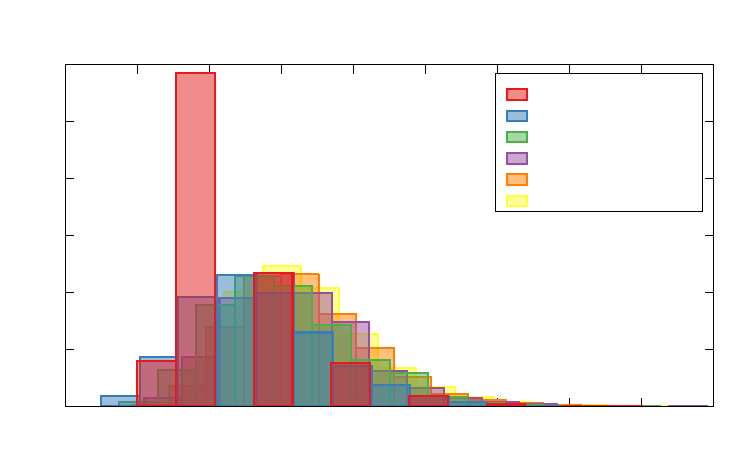
\includegraphics[width={360.00bp},height={216.00bp}]{graf8}}%
    \gplfronttext
  \end{picture}%
\endgroup
}
    \caption{Porazdelitev števil sipanj za različna razmerja $\alpha$ z~enodimenzionalnim
    približkom.}
    \label{slika10}
\end{figure}
Na grafu~\ref{slika11} sta prikazani porazdelitvi prepuščenih žarkov po kotu $\phi$ in
po kotu $\theta$. Porazdelitev po $\theta$ odbitih oziroma prepuščenih žarkov se nič
ne spremeni s~tem, ko smo v~sistem dodali ploščo. Spremembo vidimo pri porazdelitvi
po kotu $\phi$ kjer nam pri odbitih in prepuščenih kotih \emph{zmanjka} območje 
pri $\phi= \pi/2$ oziroma $\phi=3\pi/2$, se pravi ravno v~smeri, ko imamo neskončno
dolgo ploščo. Spet lahko vidimo, kar smo že prej opazili, da z~večanjem parametra 
$\alpha$ povečujemo število prepuščenih in zmanjšujemo število odbitih nevtronov.


\begin{figure}    
    \centering
    \resizebox{0.45\linewidth}{!}{% GNUPLOT: LaTeX picture with Postscript
\begingroup
  \makeatletter
  \providecommand\color[2][]{%
    \GenericError{(gnuplot) \space\space\space\@spaces}{%
      Package color not loaded in conjunction with
      terminal option `colourtext'%
    }{See the gnuplot documentation for explanation.%
    }{Either use 'blacktext' in gnuplot or load the package
      color.sty in LaTeX.}%
    \renewcommand\color[2][]{}%
  }%
  \providecommand\includegraphics[2][]{%
    \GenericError{(gnuplot) \space\space\space\@spaces}{%
      Package graphicx or graphics not loaded%
    }{See the gnuplot documentation for explanation.%
    }{The gnuplot epslatex terminal needs graphicx.sty or graphics.sty.}%
    \renewcommand\includegraphics[2][]{}%
  }%
  \providecommand\rotatebox[2]{#2}%
  \@ifundefined{ifGPcolor}{%
    \newif\ifGPcolor
    \GPcolortrue
  }{}%
  \@ifundefined{ifGPblacktext}{%
    \newif\ifGPblacktext
    \GPblacktexttrue
  }{}%
  % define a \g@addto@macro without @ in the name:
  \let\gplgaddtomacro\g@addto@macro
  % define empty templates for all commands taking text:
  \gdef\gplbacktext{}%
  \gdef\gplfronttext{}%
  \makeatother
  \ifGPblacktext
    % no textcolor at all
    \def\colorrgb#1{}%
    \def\colorgray#1{}%
  \else
    % gray or color?
    \ifGPcolor
      \def\colorrgb#1{\color[rgb]{#1}}%
      \def\colorgray#1{\color[gray]{#1}}%
      \expandafter\def\csname LTw\endcsname{\color{white}}%
      \expandafter\def\csname LTb\endcsname{\color{black}}%
      \expandafter\def\csname LTa\endcsname{\color{black}}%
      \expandafter\def\csname LT0\endcsname{\color[rgb]{1,0,0}}%
      \expandafter\def\csname LT1\endcsname{\color[rgb]{0,1,0}}%
      \expandafter\def\csname LT2\endcsname{\color[rgb]{0,0,1}}%
      \expandafter\def\csname LT3\endcsname{\color[rgb]{1,0,1}}%
      \expandafter\def\csname LT4\endcsname{\color[rgb]{0,1,1}}%
      \expandafter\def\csname LT5\endcsname{\color[rgb]{1,1,0}}%
      \expandafter\def\csname LT6\endcsname{\color[rgb]{0,0,0}}%
      \expandafter\def\csname LT7\endcsname{\color[rgb]{1,0.3,0}}%
      \expandafter\def\csname LT8\endcsname{\color[rgb]{0.5,0.5,0.5}}%
    \else
      % gray
      \def\colorrgb#1{\color{black}}%
      \def\colorgray#1{\color[gray]{#1}}%
      \expandafter\def\csname LTw\endcsname{\color{white}}%
      \expandafter\def\csname LTb\endcsname{\color{black}}%
      \expandafter\def\csname LTa\endcsname{\color{black}}%
      \expandafter\def\csname LT0\endcsname{\color{black}}%
      \expandafter\def\csname LT1\endcsname{\color{black}}%
      \expandafter\def\csname LT2\endcsname{\color{black}}%
      \expandafter\def\csname LT3\endcsname{\color{black}}%
      \expandafter\def\csname LT4\endcsname{\color{black}}%
      \expandafter\def\csname LT5\endcsname{\color{black}}%
      \expandafter\def\csname LT6\endcsname{\color{black}}%
      \expandafter\def\csname LT7\endcsname{\color{black}}%
      \expandafter\def\csname LT8\endcsname{\color{black}}%
    \fi
  \fi
    \setlength{\unitlength}{0.0500bp}%
    \ifx\gptboxheight\undefined%
      \newlength{\gptboxheight}%
      \newlength{\gptboxwidth}%
      \newsavebox{\gptboxtext}%
    \fi%
    \setlength{\fboxrule}{0.5pt}%
    \setlength{\fboxsep}{1pt}%
\begin{picture}(7200.00,5040.00)%
    \gplgaddtomacro\gplbacktext{%
      \csname LTb\endcsname%%
      \put(814,704){\makebox(0,0)[r]{\strut{}$-80$}}%
      \csname LTb\endcsname%%
      \put(814,1733){\makebox(0,0)[r]{\strut{}$-40$}}%
      \csname LTb\endcsname%%
      \put(814,2762){\makebox(0,0)[r]{\strut{}$0$}}%
      \csname LTb\endcsname%%
      \put(814,3790){\makebox(0,0)[r]{\strut{}$40$}}%
      \csname LTb\endcsname%%
      \put(814,4819){\makebox(0,0)[r]{\strut{}$80$}}%
      \csname LTb\endcsname%%
      \put(946,484){\makebox(0,0){\strut{}$0$}}%
      \csname LTb\endcsname%%
      \put(2117,484){\makebox(0,0){\strut{}$500$}}%
      \csname LTb\endcsname%%
      \put(3289,484){\makebox(0,0){\strut{}$1000$}}%
      \csname LTb\endcsname%%
      \put(4460,484){\makebox(0,0){\strut{}$1500$}}%
      \csname LTb\endcsname%%
      \put(5632,484){\makebox(0,0){\strut{}$2000$}}%
      \csname LTb\endcsname%%
      \put(6803,484){\makebox(0,0){\strut{}$2500$}}%
    }%
    \gplgaddtomacro\gplfronttext{%
      \csname LTb\endcsname%%
      \put(209,2761){\rotatebox{-270}{\makebox(0,0){\strut{}$\vec{x}_{\text{pravi}}-x^+$}}}%
      \put(3874,154){\makebox(0,0){\strut{}$t$}}%
      \csname LTb\endcsname%%
      \put(5649,4646){\makebox(0,0){\strut{}$x$ koordinata}}%
      \csname LTb\endcsname%%
      \put(5087,4184){\makebox(0,0)[l]{\strut{}Meritev}}%
      \csname LTb\endcsname%%
      \put(5087,4404){\makebox(0,0)[l]{\strut{}Akcelerometer}}%
    }%
    \gplbacktext
    \put(0,0){\includegraphics[width={360.00bp},height={252.00bp}]{graf9a}}%
    \gplfronttext
  \end{picture}%
\endgroup
}
    \resizebox{0.45\linewidth}{!}{% GNUPLOT: LaTeX picture with Postscript
\begingroup
  \makeatletter
  \providecommand\color[2][]{%
    \GenericError{(gnuplot) \space\space\space\@spaces}{%
      Package color not loaded in conjunction with
      terminal option `colourtext'%
    }{See the gnuplot documentation for explanation.%
    }{Either use 'blacktext' in gnuplot or load the package
      color.sty in LaTeX.}%
    \renewcommand\color[2][]{}%
  }%
  \providecommand\includegraphics[2][]{%
    \GenericError{(gnuplot) \space\space\space\@spaces}{%
      Package graphicx or graphics not loaded%
    }{See the gnuplot documentation for explanation.%
    }{The gnuplot epslatex terminal needs graphicx.sty or graphics.sty.}%
    \renewcommand\includegraphics[2][]{}%
  }%
  \providecommand\rotatebox[2]{#2}%
  \@ifundefined{ifGPcolor}{%
    \newif\ifGPcolor
    \GPcolortrue
  }{}%
  \@ifundefined{ifGPblacktext}{%
    \newif\ifGPblacktext
    \GPblacktexttrue
  }{}%
  % define a \g@addto@macro without @ in the name:
  \let\gplgaddtomacro\g@addto@macro
  % define empty templates for all commands taking text:
  \gdef\gplbacktext{}%
  \gdef\gplfronttext{}%
  \makeatother
  \ifGPblacktext
    % no textcolor at all
    \def\colorrgb#1{}%
    \def\colorgray#1{}%
  \else
    % gray or color?
    \ifGPcolor
      \def\colorrgb#1{\color[rgb]{#1}}%
      \def\colorgray#1{\color[gray]{#1}}%
      \expandafter\def\csname LTw\endcsname{\color{white}}%
      \expandafter\def\csname LTb\endcsname{\color{black}}%
      \expandafter\def\csname LTa\endcsname{\color{black}}%
      \expandafter\def\csname LT0\endcsname{\color[rgb]{1,0,0}}%
      \expandafter\def\csname LT1\endcsname{\color[rgb]{0,1,0}}%
      \expandafter\def\csname LT2\endcsname{\color[rgb]{0,0,1}}%
      \expandafter\def\csname LT3\endcsname{\color[rgb]{1,0,1}}%
      \expandafter\def\csname LT4\endcsname{\color[rgb]{0,1,1}}%
      \expandafter\def\csname LT5\endcsname{\color[rgb]{1,1,0}}%
      \expandafter\def\csname LT6\endcsname{\color[rgb]{0,0,0}}%
      \expandafter\def\csname LT7\endcsname{\color[rgb]{1,0.3,0}}%
      \expandafter\def\csname LT8\endcsname{\color[rgb]{0.5,0.5,0.5}}%
    \else
      % gray
      \def\colorrgb#1{\color{black}}%
      \def\colorgray#1{\color[gray]{#1}}%
      \expandafter\def\csname LTw\endcsname{\color{white}}%
      \expandafter\def\csname LTb\endcsname{\color{black}}%
      \expandafter\def\csname LTa\endcsname{\color{black}}%
      \expandafter\def\csname LT0\endcsname{\color{black}}%
      \expandafter\def\csname LT1\endcsname{\color{black}}%
      \expandafter\def\csname LT2\endcsname{\color{black}}%
      \expandafter\def\csname LT3\endcsname{\color{black}}%
      \expandafter\def\csname LT4\endcsname{\color{black}}%
      \expandafter\def\csname LT5\endcsname{\color{black}}%
      \expandafter\def\csname LT6\endcsname{\color{black}}%
      \expandafter\def\csname LT7\endcsname{\color{black}}%
      \expandafter\def\csname LT8\endcsname{\color{black}}%
    \fi
  \fi
    \setlength{\unitlength}{0.0500bp}%
    \ifx\gptboxheight\undefined%
      \newlength{\gptboxheight}%
      \newlength{\gptboxwidth}%
      \newsavebox{\gptboxtext}%
    \fi%
    \setlength{\fboxrule}{0.5pt}%
    \setlength{\fboxsep}{1pt}%
\begin{picture}(7200.00,5040.00)%
    \gplgaddtomacro\gplbacktext{%
      \csname LTb\endcsname%%
      \put(946,704){\makebox(0,0)[r]{\strut{}$-120$}}%
      \csname LTb\endcsname%%
      \put(946,1390){\makebox(0,0)[r]{\strut{}$-80$}}%
      \csname LTb\endcsname%%
      \put(946,2076){\makebox(0,0)[r]{\strut{}$-40$}}%
      \csname LTb\endcsname%%
      \put(946,2762){\makebox(0,0)[r]{\strut{}$0$}}%
      \csname LTb\endcsname%%
      \put(946,3447){\makebox(0,0)[r]{\strut{}$40$}}%
      \csname LTb\endcsname%%
      \put(946,4133){\makebox(0,0)[r]{\strut{}$80$}}%
      \csname LTb\endcsname%%
      \put(946,4819){\makebox(0,0)[r]{\strut{}$120$}}%
      \csname LTb\endcsname%%
      \put(1078,484){\makebox(0,0){\strut{}$0$}}%
      \csname LTb\endcsname%%
      \put(2223,484){\makebox(0,0){\strut{}$500$}}%
      \csname LTb\endcsname%%
      \put(3368,484){\makebox(0,0){\strut{}$1000$}}%
      \csname LTb\endcsname%%
      \put(4513,484){\makebox(0,0){\strut{}$1500$}}%
      \csname LTb\endcsname%%
      \put(5658,484){\makebox(0,0){\strut{}$2000$}}%
      \csname LTb\endcsname%%
      \put(6803,484){\makebox(0,0){\strut{}$2500$}}%
    }%
    \gplgaddtomacro\gplfronttext{%
      \csname LTb\endcsname%%
      \put(209,2761){\rotatebox{-270}{\makebox(0,0){\strut{}$\vec{y}_{\text{pravi}}-y^+$}}}%
      \put(3940,154){\makebox(0,0){\strut{}$t$}}%
      \csname LTb\endcsname%%
      \put(5649,4646){\makebox(0,0){\strut{}$y$ koordinata}}%
      \csname LTb\endcsname%%
      \put(5087,4184){\makebox(0,0)[l]{\strut{}Meritev}}%
      \csname LTb\endcsname%%
      \put(5087,4404){\makebox(0,0)[l]{\strut{}Akcelerometer}}%
    }%
    \gplbacktext
    \put(0,0){\includegraphics[width={360.00bp},height={252.00bp}]{graf9b}}%
    \gplfronttext
  \end{picture}%
\endgroup
}
    \caption{Kotna porazdelitev prepuščenih žarkov.}
    \label{slika11}
\end{figure}

\begin{figure}    
    \centering
    \resizebox{0.45\linewidth}{!}{% GNUPLOT: LaTeX picture with Postscript
\begingroup
  \makeatletter
  \providecommand\color[2][]{%
    \GenericError{(gnuplot) \space\space\space\@spaces}{%
      Package color not loaded in conjunction with
      terminal option `colourtext'%
    }{See the gnuplot documentation for explanation.%
    }{Either use 'blacktext' in gnuplot or load the package
      color.sty in LaTeX.}%
    \renewcommand\color[2][]{}%
  }%
  \providecommand\includegraphics[2][]{%
    \GenericError{(gnuplot) \space\space\space\@spaces}{%
      Package graphicx or graphics not loaded%
    }{See the gnuplot documentation for explanation.%
    }{The gnuplot epslatex terminal needs graphicx.sty or graphics.sty.}%
    \renewcommand\includegraphics[2][]{}%
  }%
  \providecommand\rotatebox[2]{#2}%
  \@ifundefined{ifGPcolor}{%
    \newif\ifGPcolor
    \GPcolortrue
  }{}%
  \@ifundefined{ifGPblacktext}{%
    \newif\ifGPblacktext
    \GPblacktexttrue
  }{}%
  % define a \g@addto@macro without @ in the name:
  \let\gplgaddtomacro\g@addto@macro
  % define empty templates for all commands taking text:
  \gdef\gplbacktext{}%
  \gdef\gplfronttext{}%
  \makeatother
  \ifGPblacktext
    % no textcolor at all
    \def\colorrgb#1{}%
    \def\colorgray#1{}%
  \else
    % gray or color?
    \ifGPcolor
      \def\colorrgb#1{\color[rgb]{#1}}%
      \def\colorgray#1{\color[gray]{#1}}%
      \expandafter\def\csname LTw\endcsname{\color{white}}%
      \expandafter\def\csname LTb\endcsname{\color{black}}%
      \expandafter\def\csname LTa\endcsname{\color{black}}%
      \expandafter\def\csname LT0\endcsname{\color[rgb]{1,0,0}}%
      \expandafter\def\csname LT1\endcsname{\color[rgb]{0,1,0}}%
      \expandafter\def\csname LT2\endcsname{\color[rgb]{0,0,1}}%
      \expandafter\def\csname LT3\endcsname{\color[rgb]{1,0,1}}%
      \expandafter\def\csname LT4\endcsname{\color[rgb]{0,1,1}}%
      \expandafter\def\csname LT5\endcsname{\color[rgb]{1,1,0}}%
      \expandafter\def\csname LT6\endcsname{\color[rgb]{0,0,0}}%
      \expandafter\def\csname LT7\endcsname{\color[rgb]{1,0.3,0}}%
      \expandafter\def\csname LT8\endcsname{\color[rgb]{0.5,0.5,0.5}}%
    \else
      % gray
      \def\colorrgb#1{\color{black}}%
      \def\colorgray#1{\color[gray]{#1}}%
      \expandafter\def\csname LTw\endcsname{\color{white}}%
      \expandafter\def\csname LTb\endcsname{\color{black}}%
      \expandafter\def\csname LTa\endcsname{\color{black}}%
      \expandafter\def\csname LT0\endcsname{\color{black}}%
      \expandafter\def\csname LT1\endcsname{\color{black}}%
      \expandafter\def\csname LT2\endcsname{\color{black}}%
      \expandafter\def\csname LT3\endcsname{\color{black}}%
      \expandafter\def\csname LT4\endcsname{\color{black}}%
      \expandafter\def\csname LT5\endcsname{\color{black}}%
      \expandafter\def\csname LT6\endcsname{\color{black}}%
      \expandafter\def\csname LT7\endcsname{\color{black}}%
      \expandafter\def\csname LT8\endcsname{\color{black}}%
    \fi
  \fi
    \setlength{\unitlength}{0.0500bp}%
    \ifx\gptboxheight\undefined%
      \newlength{\gptboxheight}%
      \newlength{\gptboxwidth}%
      \newsavebox{\gptboxtext}%
    \fi%
    \setlength{\fboxrule}{0.5pt}%
    \setlength{\fboxsep}{1pt}%
\begin{picture}(7200.00,5040.00)%
    \gplgaddtomacro\gplbacktext{%
      \csname LTb\endcsname%%
      \put(946,704){\makebox(0,0)[r]{\strut{}$-240$}}%
      \csname LTb\endcsname%%
      \put(946,1078){\makebox(0,0)[r]{\strut{}$-200$}}%
      \csname LTb\endcsname%%
      \put(946,1452){\makebox(0,0)[r]{\strut{}$-160$}}%
      \csname LTb\endcsname%%
      \put(946,1826){\makebox(0,0)[r]{\strut{}$-120$}}%
      \csname LTb\endcsname%%
      \put(946,2200){\makebox(0,0)[r]{\strut{}$-80$}}%
      \csname LTb\endcsname%%
      \put(946,2574){\makebox(0,0)[r]{\strut{}$-40$}}%
      \csname LTb\endcsname%%
      \put(946,2949){\makebox(0,0)[r]{\strut{}$0$}}%
      \csname LTb\endcsname%%
      \put(946,3323){\makebox(0,0)[r]{\strut{}$40$}}%
      \csname LTb\endcsname%%
      \put(946,3697){\makebox(0,0)[r]{\strut{}$80$}}%
      \csname LTb\endcsname%%
      \put(946,4071){\makebox(0,0)[r]{\strut{}$120$}}%
      \csname LTb\endcsname%%
      \put(946,4445){\makebox(0,0)[r]{\strut{}$160$}}%
      \csname LTb\endcsname%%
      \put(946,4819){\makebox(0,0)[r]{\strut{}$200$}}%
      \csname LTb\endcsname%%
      \put(1078,484){\makebox(0,0){\strut{}$0$}}%
      \csname LTb\endcsname%%
      \put(2223,484){\makebox(0,0){\strut{}$500$}}%
      \csname LTb\endcsname%%
      \put(3368,484){\makebox(0,0){\strut{}$1000$}}%
      \csname LTb\endcsname%%
      \put(4513,484){\makebox(0,0){\strut{}$1500$}}%
      \csname LTb\endcsname%%
      \put(5658,484){\makebox(0,0){\strut{}$2000$}}%
      \csname LTb\endcsname%%
      \put(6803,484){\makebox(0,0){\strut{}$2500$}}%
    }%
    \gplgaddtomacro\gplfronttext{%
      \csname LTb\endcsname%%
      \put(209,2761){\rotatebox{-270}{\makebox(0,0){\strut{}$\vec{x}_{\text{pravi}}-x^+$}}}%
      \put(3940,154){\makebox(0,0){\strut{}$t$}}%
      \csname LTb\endcsname%%
      \put(5583,1779){\makebox(0,0){\strut{}$x$ koordinata}}%
      \csname LTb\endcsname%%
      \put(4955,877){\makebox(0,0)[l]{\strut{}Meritev}}%
      \csname LTb\endcsname%%
      \put(4955,1097){\makebox(0,0)[l]{\strut{}Akcelerometer$^2$}}%
      \csname LTb\endcsname%%
      \put(4955,1317){\makebox(0,0)[l]{\strut{}Akcelerometer$^1$}}%
      \csname LTb\endcsname%%
      \put(4955,1537){\makebox(0,0)[l]{\strut{}Akcelerometer$^0$}}%
    }%
    \gplbacktext
    \put(0,0){\includegraphics[width={360.00bp},height={252.00bp}]{graf10a}}%
    \gplfronttext
  \end{picture}%
\endgroup
}
    \resizebox{0.45\linewidth}{!}{% GNUPLOT: LaTeX picture with Postscript
\begingroup
  \makeatletter
  \providecommand\color[2][]{%
    \GenericError{(gnuplot) \space\space\space\@spaces}{%
      Package color not loaded in conjunction with
      terminal option `colourtext'%
    }{See the gnuplot documentation for explanation.%
    }{Either use 'blacktext' in gnuplot or load the package
      color.sty in LaTeX.}%
    \renewcommand\color[2][]{}%
  }%
  \providecommand\includegraphics[2][]{%
    \GenericError{(gnuplot) \space\space\space\@spaces}{%
      Package graphicx or graphics not loaded%
    }{See the gnuplot documentation for explanation.%
    }{The gnuplot epslatex terminal needs graphicx.sty or graphics.sty.}%
    \renewcommand\includegraphics[2][]{}%
  }%
  \providecommand\rotatebox[2]{#2}%
  \@ifundefined{ifGPcolor}{%
    \newif\ifGPcolor
    \GPcolortrue
  }{}%
  \@ifundefined{ifGPblacktext}{%
    \newif\ifGPblacktext
    \GPblacktexttrue
  }{}%
  % define a \g@addto@macro without @ in the name:
  \let\gplgaddtomacro\g@addto@macro
  % define empty templates for all commands taking text:
  \gdef\gplbacktext{}%
  \gdef\gplfronttext{}%
  \makeatother
  \ifGPblacktext
    % no textcolor at all
    \def\colorrgb#1{}%
    \def\colorgray#1{}%
  \else
    % gray or color?
    \ifGPcolor
      \def\colorrgb#1{\color[rgb]{#1}}%
      \def\colorgray#1{\color[gray]{#1}}%
      \expandafter\def\csname LTw\endcsname{\color{white}}%
      \expandafter\def\csname LTb\endcsname{\color{black}}%
      \expandafter\def\csname LTa\endcsname{\color{black}}%
      \expandafter\def\csname LT0\endcsname{\color[rgb]{1,0,0}}%
      \expandafter\def\csname LT1\endcsname{\color[rgb]{0,1,0}}%
      \expandafter\def\csname LT2\endcsname{\color[rgb]{0,0,1}}%
      \expandafter\def\csname LT3\endcsname{\color[rgb]{1,0,1}}%
      \expandafter\def\csname LT4\endcsname{\color[rgb]{0,1,1}}%
      \expandafter\def\csname LT5\endcsname{\color[rgb]{1,1,0}}%
      \expandafter\def\csname LT6\endcsname{\color[rgb]{0,0,0}}%
      \expandafter\def\csname LT7\endcsname{\color[rgb]{1,0.3,0}}%
      \expandafter\def\csname LT8\endcsname{\color[rgb]{0.5,0.5,0.5}}%
    \else
      % gray
      \def\colorrgb#1{\color{black}}%
      \def\colorgray#1{\color[gray]{#1}}%
      \expandafter\def\csname LTw\endcsname{\color{white}}%
      \expandafter\def\csname LTb\endcsname{\color{black}}%
      \expandafter\def\csname LTa\endcsname{\color{black}}%
      \expandafter\def\csname LT0\endcsname{\color{black}}%
      \expandafter\def\csname LT1\endcsname{\color{black}}%
      \expandafter\def\csname LT2\endcsname{\color{black}}%
      \expandafter\def\csname LT3\endcsname{\color{black}}%
      \expandafter\def\csname LT4\endcsname{\color{black}}%
      \expandafter\def\csname LT5\endcsname{\color{black}}%
      \expandafter\def\csname LT6\endcsname{\color{black}}%
      \expandafter\def\csname LT7\endcsname{\color{black}}%
      \expandafter\def\csname LT8\endcsname{\color{black}}%
    \fi
  \fi
    \setlength{\unitlength}{0.0500bp}%
    \ifx\gptboxheight\undefined%
      \newlength{\gptboxheight}%
      \newlength{\gptboxwidth}%
      \newsavebox{\gptboxtext}%
    \fi%
    \setlength{\fboxrule}{0.5pt}%
    \setlength{\fboxsep}{1pt}%
\begin{picture}(7200.00,5040.00)%
    \gplgaddtomacro\gplbacktext{%
      \csname LTb\endcsname%%
      \put(946,704){\makebox(0,0)[r]{\strut{}$-160$}}%
      \csname LTb\endcsname%%
      \put(946,1021){\makebox(0,0)[r]{\strut{}$-120$}}%
      \csname LTb\endcsname%%
      \put(946,1337){\makebox(0,0)[r]{\strut{}$-80$}}%
      \csname LTb\endcsname%%
      \put(946,1654){\makebox(0,0)[r]{\strut{}$-40$}}%
      \csname LTb\endcsname%%
      \put(946,1970){\makebox(0,0)[r]{\strut{}$0$}}%
      \csname LTb\endcsname%%
      \put(946,2287){\makebox(0,0)[r]{\strut{}$40$}}%
      \csname LTb\endcsname%%
      \put(946,2603){\makebox(0,0)[r]{\strut{}$80$}}%
      \csname LTb\endcsname%%
      \put(946,2920){\makebox(0,0)[r]{\strut{}$120$}}%
      \csname LTb\endcsname%%
      \put(946,3236){\makebox(0,0)[r]{\strut{}$160$}}%
      \csname LTb\endcsname%%
      \put(946,3553){\makebox(0,0)[r]{\strut{}$200$}}%
      \csname LTb\endcsname%%
      \put(946,3869){\makebox(0,0)[r]{\strut{}$240$}}%
      \csname LTb\endcsname%%
      \put(946,4186){\makebox(0,0)[r]{\strut{}$280$}}%
      \csname LTb\endcsname%%
      \put(946,4502){\makebox(0,0)[r]{\strut{}$320$}}%
      \csname LTb\endcsname%%
      \put(946,4819){\makebox(0,0)[r]{\strut{}$360$}}%
      \csname LTb\endcsname%%
      \put(1078,484){\makebox(0,0){\strut{}$0$}}%
      \csname LTb\endcsname%%
      \put(2223,484){\makebox(0,0){\strut{}$500$}}%
      \csname LTb\endcsname%%
      \put(3368,484){\makebox(0,0){\strut{}$1000$}}%
      \csname LTb\endcsname%%
      \put(4513,484){\makebox(0,0){\strut{}$1500$}}%
      \csname LTb\endcsname%%
      \put(5658,484){\makebox(0,0){\strut{}$2000$}}%
      \csname LTb\endcsname%%
      \put(6803,484){\makebox(0,0){\strut{}$2500$}}%
    }%
    \gplgaddtomacro\gplfronttext{%
      \csname LTb\endcsname%%
      \put(209,2761){\rotatebox{-270}{\makebox(0,0){\strut{}$\vec{y}_{\text{pravi}}-y^+$}}}%
      \put(3940,154){\makebox(0,0){\strut{}$t$}}%
      \csname LTb\endcsname%%
      \put(5583,4646){\makebox(0,0){\strut{}$y$ koordinata}}%
      \csname LTb\endcsname%%
      \put(4955,3744){\makebox(0,0)[l]{\strut{}Meritev}}%
      \csname LTb\endcsname%%
      \put(4955,3964){\makebox(0,0)[l]{\strut{}Akcelerometer$^2$}}%
      \csname LTb\endcsname%%
      \put(4955,4184){\makebox(0,0)[l]{\strut{}Akcelerometer$^1$}}%
      \csname LTb\endcsname%%
      \put(4955,4404){\makebox(0,0)[l]{\strut{}Akcelerometer$^0$}}%
    }%
    \gplbacktext
    \put(0,0){\includegraphics[width={360.00bp},height={252.00bp}]{graf10b}}%
    \gplfronttext
  \end{picture}%
\endgroup
}
    \caption{Kotna porazdelitev odbitih žarkov.}
    \label{slika12}
\end{figure}



\end{document}
